%% ===================================================================
%% Body of the iSKYLAB mixed-phase paper, draft v0.3 (17 Nov 2026).
%% Shared by main.tex (Copernicus) and standalone.tex (article).
%% Figures: figs/fig01-03 (paper_figs.py) and figs/F04-F12 (paper_figs_v3.py);
%% every number: analysis/mixed_phase/paper/numbers_v3.json
%% (ISKYLAB_TSAT=hygrometer python3 paper_figs_v3.py).
%% ===================================================================

\introduction

Mixed-phase clouds contain supercooled droplets and ice crystals together. Because the saturation vapour pressure over ice is lower than over liquid water, a few ice crystals can grow at the expense of many droplets, so the number of crystals that form first largely decides how quickly a mixed-phase cloud glaciates, precipitates and changes its radiative properties. Between about $0$ and $-38\,^\circ$C ice forms on ice-nucleating particles (INPs), of which mineral dust is the most abundant and best characterised \citep{Hoose2012,Murray2012,Kanji2017}. Most dust is thought to freeze by immersion freezing, from within a supercooled droplet \citep{Vali2015}, and the parameterisations used in models give the ice-nucleation active-site density, \ns, of dust immersed in water at water saturation \citep{Niemand2012,Ullrich2017}.

If dust must first become a cloud droplet before it can freeze, then anything that changes droplet activation also changes ice formation. Hygroscopic particles such as sea salt activate at lower supersaturations than uncoated dust \citep{Kumar2011}, take up the vapour made available by the cooling, and can hold the supersaturation below that needed to activate the dust. \citet{Simpson2018} used a bin-microphysics parcel model to show that such cloud condensation nuclei can outcompete INPs for water vapour and so suppress ice formation, and that the size of the suppression depends on how much condensed water an INP needs before it can freeze: strong if dust must activate to a droplet, weak if a thin film of water is enough. That requirement is not known. Dust takes up water by adsorption well below water saturation \citep{Kumar2009,Kumar2011}, and dust nucleates ice below water saturation in what has been called condensation or deposition freezing \citep{Moehler2006,Field2006,Hoose2012}, possibly by freezing of water held in pores and cavities \citep{Marcolli2014}. Where dust and sea salt meet --- over the oceans downwind of deserts and arid soils, in coastal air, and in proposals for marine cloud brightening \citep{Connolly2014} --- the answer decides whether the salt reduces the ice in mixed-phase clouds.

A cloud chamber can test this directly, because the aerosol is known and the same expansion can be repeated with and without the competing salt. In the iSKYLAB campaign (improved Scientific Knowledge of Clouds, Ice CrYstals, and Aerosols through LABoratory Access of a New Dynamic Cloud Chamber), in the AIDAd chamber (AIDA, Aerosol Interactions and Dynamics in the Atmosphere; d, dynamic) at the Karlsruhe Institute of Technology (KIT), we carried out warm-cloud experiments with ammonium sulfate, fulvic acid and NaCl, and mixed-phase experiments with two dusts, alone and mixed with NaCl. The warm-cloud experiments are analysed in a companion paper \citep[hereafter Paper~1]{Connolly2026}. Paper~1 showed that with the mixing fan running the AIDAd cloud is controlled by its walls: air conditioned at the wall mixes into the chamber every 10\,s or so and evaporates the smallest droplets, and by holding the air close to water saturation the walls strengthen the competition between aerosols for droplet formation. It also showed that the WELAS optical particle counter misses small droplets, which evaporate in its warm inlet, so that this competition could be simulated but not observed.

The mixed-phase experiments offer a cleaner observable. Ice crystals grow to tens of micrometres, and the question becomes: when NaCl takes the water vapour and the dust does not form droplets, does the dust still freeze? Because the dust and the NaCl were injected as separate particles, the NaCl can affect the dust only through the vapour it takes up and the cloud it makes; it does not coat the dust. Section~\ref{sec:experiments} describes the experiments, Sect.~\ref{sec:model} the model and how it was constrained, Sect.~\ref{sec:obs} what was observed, Sect.~\ref{sec:test} the test of two hypotheses for when dust can freeze, and Sect.~\ref{sec:mech} what the salt does in the model. Section~\ref{sec:discussion} discusses what the experiments can and cannot show about the atmosphere.

%% ------------------------------------------------------------------
\section{Experiments}\label{sec:experiments}

\subsection{The AIDAd chamber and its instruments}

The AIDAd cloud vessel, of aluminium (3.8\,m$^3$, 2.15\,m high, 1.50\,m in diameter), and its instruments are described in Paper~1 and \citet{Alpert2023}. The vessel sits inside a stainless-steel vacuum vessel and is pumped through a controlled valve, so that the gas cools as the pressure falls while the wall segments are cooled at the same rate. A two-blade carbon-fibre propeller of 33\,cm diameter, on the axis of the vessel and reaching 30--40\,cm into it through the top flange, mixes the gas; it ran in all experiments reported here, at an unmeasured rate of 3600--6200\,rpm. The gas temperature and the wall temperatures are measured with thermocouples; the frost and dew points of the total water (vapour plus condensate) with an MBW chilled-mirror hygrometer; the total particle number with a condensation particle counter (CPC); and particles between 0.3 and about 218\um\ with two WELAS optical particle counters (2300P and 2500P), whose data are merged by KIT. WELAS reports an optical, scattering-equivalent diameter calculated for a water sphere (refractive index 1.33). Both WELAS sample at 5\,L\,min$^{-1}$ through vertical lines that enter through the bottom of the vessel, 30\,cm (2500P) and 50\,cm (2300P) from its axis. Each line runs about 10\,cm inside the vessel, about 50\,cm through the space between the cloud vessel and the vacuum vessel, where the gas is warmer than in the cloud vessel, and about 15\,cm through the laboratory to the sensor, so droplets partly evaporate on the way (Paper~1). INP spectra were measured with the INSEKT filter method (Ice Nucleation SpEctrometer of the Karlsruhe Institute of Technology) in all six experiments \todo{KIT: INSEKT sampling (time, volume, temperature range) and whether the spectra can be included; see Sect.~\ref{sec:disc-residual}}.

In the merged WELAS files KIT classify particles larger than 15\um\ as ice (NIce) and particles of 0.3--15\um\ as droplets or aerosol (NDrop). Once ice is present the size distributions have a gap between about 15 and 25\um\ (Fig.~\ref{fig:spectra}), so the observed ice count is not sensitive to the exact threshold. \todo{KIT (RW, NSU): confirm the ice--droplet separation (size only, or also depolarisation or asphericity?), whether ice smaller than 15\um\ would be counted in NDrop, and the transmission of the inlet for crystals larger than 50\um}

\subsection{Aerosols and the experiment sequence}

Table~\ref{tab:experiments} lists the six experiments, made on 19--21 June 2024. Two dusts were used: a soil dust from the Succulent Karoo biome in South Africa (SDSA01; \citealp{Bazo2026}) \todo{KIT: confirm the SDSA01 reference} and Arizona test dust (ATD03). Each dust was first injected alone (Exp021, Exp025) and then together with NaCl particles atomised from a 0.1\,wt\,\% solution (Exp022 and Exp023 with SDSA01; Exp026 and Exp027 with ATD03). Dust and NaCl were injected separately, so they were externally mixed. Two further dust experiments are not analysed: Exp020 (SDSA01) is not in the data set, and Exp024 (a second dust, SDTP02) was cooled at 2\,K\,min$^{-1}$ \todo{KIT: Exp020 and Exp024 data, if available; Exp020 would give a second SDSA01-alone experiment}.

KIT separated the measured initial size distribution (SMPS and APS, merged on a volume-equivalent diameter grid assuming a density of 2.6\,g\,cm$^{-3}$ and a dynamic shape factor of 1.5) into its dust and NaCl components (Fig.~\ref{fig:aerosol}), and we use this split throughout. The mixtures contained less dust than the dust-alone experiments: 405--472\cmc\ of SDSA01 in Exp022 and Exp023 against 1160\cmc\ in Exp021, and 791--889\cmc\ of ATD03 in Exp026 and Exp027 against 1190\cmc\ in Exp025. Their dust surface area was 42--50\,\% (SDSA01) and 76--77\,\% (ATD03) of that in the dust-alone experiments. NaCl dominated the number (3970--10\,500\cmc). Comparisons between experiments with and without NaCl therefore include the effect of the different amounts of dust. We account for it by normalising the observed ice by the dust surface and by simulating each experiment with its own measured aerosol.

All six expansions started at gas temperatures of $-11.3$ to $-13.5\,^\circ$C and pressures of 978--986\,hPa (934\,hPa in Exp022), with relative humidities of 69--79\,\% over water (77--88\,\% over ice), and cooled at 0.5\,K\,min$^{-1}$ to about $-30\,^\circ$C over 33--39\,min. The hygrometer reached water saturation 8.2--12.3\,min after the start of pumping, at $-16.7$ to $-20.1\,^\circ$C (Table~\ref{tab:experiments}). We use this time, $t_\mathrm{sat}$, as the start of the cloud in both observations and model.

\subsection{Ice-nucleation active-site density from the observations}\label{sec:ns}

We calculated the active-site density from the observations ourselves,
\begin{equation}
  \ns(t) = \frac{N_\mathrm{ice}(t)}{S_\mathrm{dust}(0)\,f(t)},
  \label{eq:ns}
\end{equation}
where $N_\mathrm{ice}$ is the WELAS ice number smoothed over 31\,s, $S_\mathrm{dust}(0)$ the dust surface concentration at the start of the expansion from KIT's dust component, and $f(t)$ the ratio of the CPC number to its starting value, which accounts for dilution and loss of particles. The values are binned in 0.5\,K intervals of gas temperature. Crystals that have fallen out are not counted, so Eq.~(\ref{eq:ns}) is a lower bound on the cumulative \ns. For the mixtures, dividing by the dust surface alone assumes that NaCl does not nucleate ice; deliquesced NaCl does not, and crystalline NaCl and its dihydrate nucleate ice only below about $-45\,^\circ$C \citep{Wagner2013,Wagner2018}.

%% ------------------------------------------------------------------
\section{Model}\label{sec:model}

\subsection{What is carried over from the warm-cloud experiments}

We use the bin-microphysics model (BMM) and chamber configuration of Paper~1 (Table~\ref{tab:model}), driven by the measured pressure, gas temperature and wall temperature. Each aerosol type is an external mode of 60 aerosol bins, with 80 bins appended for the condensed phase; particles move freely in size, and water uptake by NaCl follows $\kappa$-K\"ohler theory with $\kappa = 1.28$ \citep{Petters2007}. Particles are lost to the walls following \citet{LaiNazaroff2000} and fall out at a rate $V_t/H$ with $H = 2.15$\,m.

The walls act on the chamber air in two ways. First, as in Paper~1, every time step a fraction $1-\exp(-\Delta t/\tau_\mathrm{BL})$ of the chamber air, with $\tau_\mathrm{BL} = 10$\,s, is replaced by air brought to the temperature
\begin{equation}
  T_\mathrm{BL} = T_\mathrm{gas} + \dTBL ,
  \label{eq:tbl}
\end{equation}
and droplets in that air are evaporated preferentially from the small end of the spectrum (size exponent $p = 2$). How \dTBL\ is chosen is described in Sect.~\ref{sec:wall}. Second, water vapour is exchanged with the walls at a finite rate (Sect.~\ref{sec:start}). This differs from Paper~1, which caps the humidity of the air that visits the wall at saturation at $T_\mathrm{BL}$, so that vapour is removed as fast as the air reaches the wall; Paper~1 tested a finite-rate flux at the measured wall temperature and found that it reproduces neither the water lost before the warm clouds nor the clouds themselves (its Sect.~4.7). The walls were different in the two sets of experiments: in the warm experiments they were near 0\,$^\circ$C and colder than the gas; here they were at $-12$ to $-30\,^\circ$C and, during the cloud, 0.03--0.34\,K warmer than the gas, and the model treats them as ice. In BMM this is the wall-water mode \texttt{chamber\_bl\_wall\_water\_mode = 2} (Paper~1 uses mode~0).

\subsection{Starting humidity and loss of water to the walls}\label{sec:start}

Paper~1 starts its model drier than measured and fits the time of cloud formation, so that modelled liquid appears when WELAS first detects liquid; the drier start accounts for 76\,\% of the total water that the hygrometer loses before the warm clouds. Here we model that loss instead. The model starts from the relative humidity measured by the hygrometer at the start of pumping (Table~\ref{tab:experiments}) and from the aerosol measured at that time, and water vapour is exchanged with the walls at a finite rate:
\begin{equation}
  J_\mathrm{v} = k_\mathrm{m}\,\frac{e_\mathrm{eq}(T_\mathrm{wall}) - e}{R_\mathrm{v}\,T_\mathrm{gas}},
  \label{eq:wallflux}
\end{equation}
where $J_\mathrm{v}$ is the vapour mass flux per unit wall area (positive from the wall to the air), $e$ the vapour pressure of the air that visits the wall, $e_\mathrm{eq}$ the equilibrium vapour pressure over ice at the measured wall temperature, $R_\mathrm{v}$ the gas constant for water vapour and $k_\mathrm{m}$ a transfer velocity. The measured wall temperature stayed between $-11.8$ and $-30\,^\circ$C in all six experiments, so the wall is always ice in the model. The wall starts dry: it can always take up vapour, but can return only water it has taken up.

We fitted $k_\mathrm{m}$ to the total water measured by the hygrometer from 1\,min after the start of pumping to $t_\mathrm{sat}$, before any cloud (Fig.~\ref{fig:wallsink}). A single value, $k_\mathrm{m} = 3\times10^{-4}$\,m\,s$^{-1}$, reproduces all six experiments to within 0.4--0.6 percentage points of relative humidity (root mean square), against 0.9--1.2 points for $1\times10^{-4}$ and for $8\times10^{-4}$\,m\,s$^{-1}$. A value of $5\times10^{-4}$\,m\,s$^{-1}$ fits this period as well (0.3--0.5 points) but delays the cloud onset by 0.6--1.8\,min; we use $3\times10^{-4}$\,m\,s$^{-1}$ in all simulations. The time of cloud onset is then a prediction: in the final simulations the modelled total water reaches water saturation 12--30\,s before the hygrometer does in five experiments, and 18\,s after it in Exp021 (mode~1; Table~\ref{tab:experiments}), that is within 0.1--0.25\,K of cooling.

The fit depends on the flux, not only on the starting humidity. In three experiments (Exp021, Exp025, Exp027) we reran the final simulations with $k_\mathrm{m} = 0$ and with 30 times the fitted value, changing nothing else. With $k_\mathrm{m} = 0$ the modelled total water does not fall before the cloud (0 to $-0.8$\,\%, against $-2.8$ to $-3.6$\,\% measured), the model reaches water saturation 62--76\,s early, and the root-mean-square difference rises to 1.2--1.5 points. With $9\times10^{-3}$\,m\,s$^{-1}$ the total water falls by 13--15\,\% and no cloud forms. The flux acts before these clouds because the walls are ice: the air becomes supersaturated over the ice wall 4--6\,min after the start of pumping, when its relative humidity over water is only 85--88\,\%, and the measured loss of total water then speeds up about three-fold (from 0.12--0.19 to 0.42--0.57\,\% per minute). Over the liquid walls of the warm experiments, near 0\,$^\circ$C, the air is not supersaturated until its relative humidity reaches 96--100\,\%, so a flux at the measured wall temperature acts only just before the cloud (Paper~1).

Two features show that $k_\mathrm{m}$ is an effective rate rather than a measured property of the wall. First, the hygrometer loses 0.5--0.9\,\% of the total water before the air becomes supersaturated over the wall, which Eq.~(\ref{eq:wallflux}) cannot do; the fitted flux compensates by removing water faster afterwards, so the modelled total water lags the measured by up to 0.9\,\% midway and matches it at $t_\mathrm{sat}$. In the warm experiments, where the flux is inactive before the cloud, the hygrometer also loses 3--5\,\% of the total water before the cloud (Paper~1); no wall model in either paper explains this early loss. Second, the fitted rate is about 1\,\% of a diffusion-limited transfer to the wall: the saturation cap of Paper~1, which brings the air that visits the wall to equilibrium every $\tau_\mathrm{BL} = 10$\,s, corresponds to $k_\mathrm{m} \approx (V/A)/\tau_\mathrm{BL} \approx 0.03$\,m\,s$^{-1}$, with $V$ and $A$ the chamber volume and wall area. Why the cold walls take up vapour about 100 times more slowly than the warm walls is not known; partial frost cover of the walls is one candidate, since the air before pumping was only 77--88\,\% saturated over ice. \todo{KIT: were the walls ice-coated before these experiments, and over what fraction of their area?}

Paper~1 also found that this flux combined with wall-conditioned air, with its own offsets, removes the total water of the warm clouds 21\,\% too fast (its Sect.~4.7). Here the offsets are fitted with the flux in place, and they come out warmer ($-0.05$ to $+0.20$\,K, against $-0.07$ to $-0.096$\,K in 12 of the 14 warm experiments of Paper~1); Section~\ref{sec:test-liquid} gives the water budget in cloud that results.

\subsection{Water uptake by the dust}

Dust takes up water by multilayer adsorption, described by Frenkel--Halsey--Hill (FHH) adsorption theory \citep{Kumar2009,Kumar2011}. The equilibrium saturation ratio over a dust particle carrying $\theta$ monolayers of water is
\begin{equation}
  S_\mathrm{w} = \exp\!\left(\frac{4\sigma_\mathrm{w} M_\mathrm{w}}{R T \rho_\mathrm{w} D}\right)\exp\!\left(-A_\mathrm{FHH}\,\theta^{-B_\mathrm{FHH}}\right),
  \label{eq:fhh}
\end{equation}
with $D$ the wet diameter. For ATD03 we use $A_\mathrm{FHH} = 2.96$, $B_\mathrm{FHH} = 1.28$, the values \citet{Kumar2011} fitted to their measurements of dry-generated Arizona test dust. For SDSA01, which has no measurement of its own, we use $A_\mathrm{FHH} = 2.25$, $B_\mathrm{FHH} = 1.20$, the single set with which \citet{Kumar2011} reproduced the CCN activity of all the regional dusts and minerals they measured. \todo{PJC: the model dust density is 4000\,kg\,m$^{-3}$; the KIT size grid assumes 2600\,kg\,m$^{-3}$. Correct and rerun, or show that it does not matter}

\subsection{Ice nucleation on the dust, calibrated inside the model}\label{sec:nsfit}

Freezing follows the singular, surface-based description. BMM implements it by storing, with each dust bin, the distribution of the particles' freezing temperatures (Fig.~\ref{fig:scheme}; Appendix~\ref{app:ns}). When the aerosol is made, each bin receives $K$ cumulative counts
\begin{equation}
  N_k = N\left\{1-\exp\!\left[-A\,\ns(T_k)\right]\right\}, \qquad k = 1,\dots,K,
  \label{eq:inas}
\end{equation}
where $N$ is the number of particles in the bin, $A$ the surface area of a sphere with the volume-equivalent diameter of the dust, and $T_k$ one of $K = 100$ threshold temperatures from $-18$ to $-30\,^\circ$C, 0.12\,K apart. $N_k$ is the number of particles whose freezing temperature is warmer than $T_k$. The counts are then carried with the particles and are never recalculated from \ns. Whenever the gas is colder than $T_k$ and the particles in the bin are eligible to freeze (Sect.~\ref{sec:hypotheses}), the particles still counted at $T_k$ freeze: they become ice crystals and are removed from $N_k$ and from all colder counts.

Three consequences matter here. First, dust that is not eligible when the gas passes its freezing temperature keeps that temperature, and freezes as soon as it becomes eligible (Fig.~\ref{fig:scheme}c,d). A scheme that tracks only the lowest temperature a bin has reached would instead lose those particles, which would exaggerate the suppression in mode~0. Second, frozen dust leaves the dust population with its freezing temperature, so the most active sites are used up and \ns\ can be held constant colder than the fitted range without counting them twice. Third, dust that falls out inside droplets takes its stored freezing temperatures with it, which is why keeping the dust airborne changes the ice (Sect.~\ref{sec:mech}).

We take \ns(T) for each dust from its own dust-alone experiment rather than from a published fit (Fig.~\ref{fig:ns}). The published ATD fit gives 14--110 times more active sites than Exp025 between $-18.75$ and $-21.75\,^\circ$C, and in the model this made too many crystals form two or three degrees before the observed ice, which then dried out the simulated chamber. We fitted $\ln\ns$ linearly in temperature over the range where the observed \ns\ rises cleanly:
\begin{align}
  \text{SDSA01 (Exp021, } -20.75 \text{ to } -27.75\,^\circ\mathrm{C}):&\quad \ln(\ns/\mathrm{m^{-2}}) = -0.7640\,T + a_\mathrm{SDSA}, \label{eq:ns_sdsa}\\
  \text{ATD03 (Exp025, } -21.75 \text{ to } -24.75\,^\circ\mathrm{C}):&\quad \ln(\ns/\mathrm{m^{-2}}) = -1.5437\,T + a_\mathrm{ATD}, \label{eq:ns_atd}
\end{align}
with $T$ in $^\circ$C and \ns = 0 above $-18\,^\circ$C. Colder than the fitted range we hold \ns\ constant: the most active sites have been used up, and the model removes dust that has already frozen, so no further increase is needed.

The observed \ns\ (Eq.~\ref{eq:ns}) counts only the crystals still airborne, whereas the model uses \ns\ for all the ice that forms and then removes crystals by fall-out. Using the observed \ns\ directly would therefore make the model's airborne ice too low. We corrected for this inside the model: in the dust-alone simulations we computed the airborne fraction of all ice formed, $f_\mathrm{air}(T)$, and multiplied the fitted \ns\ by a single factor $F$, the median of $1/f_\mathrm{air}$ over the fitted range. This keeps the observed slope and changes only the intercept: $F = 5.5$ for SDSA01 and 2.9 for ATD03 in mode~1 (5.2 and 3.0 in mode~0; $a_\mathrm{SDSA} = 4.333$ and $a_\mathrm{ATD} = -12.453$ in mode~1). With this calibration the modelled airborne ice in the dust-alone experiments is 1.2--1.4 times the observed between $-21$ and $-26\,^\circ$C (Sect.~\ref{sec:matched}).

Calibrating on the dust-alone experiments has a consequence that must be kept in mind. The dust-alone experiments are no longer an independent test of the ice nucleation; they fix it. The test is the mixtures: with the same dust and the same \ns, does the model reproduce what the NaCl did?

\subsection{When can a dust particle freeze? Two hypotheses}\label{sec:hypotheses}

Which particles are eligible to freeze holds the hypothesis under test.

\paragraph{Mode~0: dust must activate.} Only dust particles that have activated to cloud droplets (grown beyond their critical size on the FHH curve, Eq.~\ref{eq:fhh}) can freeze. This is the usual assumption for immersion freezing, and the limit in which \citet{Simpson2018} found the strongest suppression.

\paragraph{Mode~1: wetted dust can freeze.} Any dust particle whose adsorbed water is at least a fraction $X_\mathrm{th}$ of its dry volume can freeze with the same \ns. We use $X_\mathrm{th} = 0.01$, which a 1\um\ ATD particle reaches at about 75\,\% relative humidity. $X_\mathrm{th}$ plays the role of the condensed-water requirement of \citet{Simpson2018}, expressed relative to the dry volume. Mode~1 does not lower \ns\ below water saturation \citep{Koop2000,KnopfAlpert2013}; Sect.~\ref{sec:discussion} discusses this. \todo{PJC: mode~1 with $X_\mathrm{th} = 0.1$ and 1 for the ATD03 experiments (Sect.~\ref{sec:disc-residual})}

In both modes the crystals grow by vapour diffusion with an evolving habit \citep{ChenLamb1994habit} and fall at the speeds of \citet{HeymsfieldWestbrook2010}. Mode~1 removes no water from the dust that mode~0 would keep: the two modes differ only in which dust may freeze.

\subsection{Wall-conditioned air}\label{sec:wall}

The cloud is very sensitive to \dTBL: 0.01\,K changes the steady supersaturation by about 0.08\,\%. The thermocouples that measure the wall--gas difference are uncertain to about $\pm0.15$\,K, so \dTBL\ cannot be predicted from them to the precision needed (Paper~1). We therefore fit \dTBL\ for each experiment, as in Paper~1, under two rules fixed before the ice was compared:
\begin{enumerate}
\item \textbf{\dTBL\ is fitted to the liquid phase only.} For the dust-alone experiments the fit minimises $|\ln(N_\mathrm{mod}/N_\mathrm{obs})| + |\ln(L_\mathrm{mod}/L_\mathrm{obs})|$, where $N$ is the number of droplets above the pre-cloud count, per mg of air so that the fall in air density during the expansion is not counted as a loss of droplets, and $L$ the liquid water, both as WELAS would see them (Sect.~\ref{sec:operators}), averaged over the 10\,min after $t_\mathrm{sat}$. For the mixtures, whose condensate WELAS mostly cannot see (Sect.~\ref{sec:obs-liquid}), the fit uses the total water from the hygrometer instead of $L$: $|\ln(W_\mathrm{mod}/W_\mathrm{obs})| + |\ln[(N_\mathrm{mod}+20)/(N_\mathrm{obs}+20)]|$, where $W$ is the mean excess of total water over water saturation \citep[saturation vapour pressures from][]{MurphyKoop2005}. Because the ice removes liquid, the fit is made separately for each freezing mode.
\item \textbf{The wall-conditioned air must lie between the gas and the wall temperature}, within the thermocouple uncertainty: $\min(0,\Delta T_\mathrm{wg}) - 0.15\,\mathrm{K} \le \dTBL \le \max(0,\Delta T_\mathrm{wg}) + 0.15\,\mathrm{K}$, with $\Delta T_\mathrm{wg}$ the measured wall--gas difference.
\end{enumerate}
We searched in steps of 0.05\,K. Any offset whose score lies within 0.3 of the best is treated as an acceptable fit, and the main results are given over all acceptable fits. The fitted offsets lie between $-0.05$ and $+0.20$\,K (Table~\ref{tab:experiments}, Fig.~\ref{fig:wall}), all within the measured gas--wall range. \todo{KIT: thermocouple accuracy and positions}

\subsection{Observation operators}\label{sec:operators}

The WELAS inlet operator of Paper~1 is applied to the model droplets: a droplet of diameter $D$ is counted at
\begin{equation}
  D_\mathrm{obs} = \left(D^2 - \Delta D^2\right)^{1/2}
  \label{eq:inlet}
\end{equation}
and not at all if $D^2 < \Delta D^2$. For the cold runs we use $\Delta D^2 = 25\,\mu$m$^2$, our estimate for air at about $-20\,^\circ$C carried into an instrument at room temperature; Paper~1 fitted 24\,$\mu$m$^2$ to the warm runs. We count droplets of 0.39--13\um\ above the pre-cloud count, whereas Paper~1 counts droplets larger than 2.5\um: in the mixtures WELAS saw almost no droplets of any size above the pre-cloud count (Sect.~\ref{sec:obs-liquid}), and the upper limit must stay below the 15\um\ at which particles are counted as ice.

WELAS sizes a crystal by the light it scatters, not by its maximum dimension. For particles much larger than the wavelength, the scattered light follows the projected area, so we count model crystals by the diameter of the circle with the same orientation-averaged projected area as the model crystal (a spheroid with the model's maximum dimension and aspect ratio; for any convex body the mean projected area is a quarter of the surface area). Model ice is the number of crystals with this diameter between 15 and 218\um, the observed ice range. As bounds we also count by the volume-equivalent diameter (from the crystal mass and a density of 917\,kg\,m$^{-3}$) and by the maximum dimension, and as a sensitivity test by a lower threshold of 20\um.

\subsection{Simulations and how they are compared}\label{sec:sims}

For each experiment and freezing mode we ran the model over the range of offsets above (60 simulations), and for each mixture and mode the simulation at the chosen offset with the NaCl removed and the dust unchanged (8 simulations).

\paragraph{Comparison at matched temperature (main).} With singular freezing, the ice formed on a given dust depends on its surface and on the lowest temperature reached. The mixtures and the dust-alone experiments glaciated at different temperatures (Sect.~\ref{sec:obs-ice}), so averages over a time window compare different temperature ranges. We therefore compare ice at the same gas temperature, on a 0.5\,K grid from $-21\,^\circ$C to the warmer of the observed and modelled (mode~1) glaciation, where the observed ice exceeds 0.02\cmc. For each experiment we form the ratio of observed to modelled ice, $O/M$, as a geometric mean over the grid. Mode~1 carries each experiment's dust surface, losses, temperature history and cloud, but contains no effect of the NaCl on freezing (Sect.~\ref{sec:test-m1}). The effect of the NaCl that the model does not contain is then
\begin{equation}
  E = \frac{(O/M)_\mathrm{mixture}}{(O/M)_\mathrm{dust\ alone}} .
  \label{eq:E}
\end{equation}
As a check that needs no model, we also form the ratio of the observed ice per unit dust surface in a mixture to that with the dust alone, at the same temperatures, $E_\mathrm{obs}$.

\paragraph{Window means (secondary).} For comparison with draft~0.2 and with other studies we also give the ratio of the mean ice in a mixture to that with the same dust alone, $R$, from $t_\mathrm{sat}$ to the observed end of the liquid phase, and from $t_\mathrm{sat}+5$\,min to the end of the expansion.

\paragraph{Paired simulations (model only).} The ratio of ice in a mixture simulation to that in the same simulation with the NaCl removed, $P$, isolates what the NaCl does in the model. It cannot be observed.

The test: a hypothesis is inconsistent with a mixture if the residual effect lies outside a factor of 2 of unity ($E < 0.5$ or $E > 2$) for every acceptable fit. The factor of 2, the criterion of draft~0.2, allows for the uncertainty in the dust--NaCl split, in the ice-size operator and in the calibration. For mode~0, whose mixtures form almost no ice, we compare the ice directly.

%% ------------------------------------------------------------------
\section{What was observed}\label{sec:obs}

\subsection{With NaCl, the condensed water was on particles WELAS could not see}\label{sec:obs-liquid}

With dust alone a cloud formed at $-18$ to $-20\,^\circ$C: WELAS detected 106--112 droplets per mg of air above the pre-cloud count, averaged over the 10\,min after $t_\mathrm{sat}$ (peaks of 169--190 per mg), and up to 0.03--0.04\,g\,m$^{-3}$ of liquid water (Fig.~\ref{fig:overview}c,d). With NaCl the picture was different. In Exp022, Exp023 and Exp027 WELAS detected only 8--12 droplets per mg above the pre-cloud count over the same period (peaks of 39--131 per mg), about ten times fewer than with dust alone, and at most 0.001\,g\,m$^{-3}$ of liquid water. The peaks are 1.4--1.7 times the number of NaCl particles larger than 0.5\um\ (27--77 per mg), so these droplets can have formed on the largest NaCl particles. Exp026, with the least NaCl, showed a droplet mode (65 per mg; peak 268 per mg), ten times the number of its NaCl particles larger than 0.5\um. The size distributions show the change (Fig.~\ref{fig:spectra}): with dust alone a droplet mode at 5--12\um\ grew out of the aerosol; with NaCl the distribution rose as a broad plateau between 1 and 7\um.

The hygrometer, however, saw a similar excess of total water in all six experiments, peaking at 107--114\,\% of water saturation (Fig.~\ref{fig:overview}a,b), so all six held of order 0.1\,g\,m$^{-3}$ of condensed water. In the mixtures this water was therefore mostly on particles that do not survive the WELAS inlet (Eq.~\ref{eq:inlet}): particles smaller than about 5\um.

\subsection{At the same temperature, the SDSA01 mixtures formed more ice than the dust alone, and the ATD03 mixtures less}\label{sec:obs-ice}

Ice appeared in all six experiments at about $-20$ to $-21\,^\circ$C, after the hygrometer had reached water saturation; in no experiment was ice above the background of about 0.02\cmc\ before $t_\mathrm{sat}$. Figure~\ref{fig:matched}a,b shows the observed ice per unit dust surface against gas temperature, up to the end of the liquid phase.

For ATD03 the mixtures formed less ice per unit dust surface than the dust alone at the same temperature: $E_\mathrm{obs} = 0.51$ (Exp026) and 0.89 (Exp027), geometric means over 6 and 8 temperatures between $-21$ and $-24.5\,^\circ$C (Table~\ref{tab:matched}). Without normalising by the dust surface the ratios are 0.38 and 0.69.

For SDSA01 the mixtures formed more: $E_\mathrm{obs} = 5.3$ (Exp022) and 6.6 (Exp023), over 8 and 7 temperatures between $-21.5$ and $-25\,^\circ$C, and 2.6 and 2.7 without normalising, although the mixtures held 0.42--0.50 of the dust surface. The extra counts are crystals: at $-23$ and $-24\,^\circ$C more than 90\,\% of the particles counted as ice in the SDSA01 mixtures were larger than 40\um, while the droplets had a median optical diameter of 1--2\um. The ATD03 mixtures, which held similar amounts of the same NaCl, show no such excess, so the extra ice is not an artefact of the NaCl itself.

\subsection{Glaciation, and the fall of the observed ice after it}\label{sec:obs-glac}

The liquid phase ended (WELAS liquid water below 10\,\% of its peak) at $-24.7$ to $-25.1\,^\circ$C in the three ATD03 experiments and in both SDSA01 mixtures, but only at $-28.0\,^\circ$C in Exp021 (Fig.~\ref{fig:mechanisms}c). The SDSA01 mixtures therefore glaciated three degrees warmer than the dust alone, with half the dust surface, which agrees independently of the ice count with more ice forming in them. After glaciation the observed ice fell, by factors of 7--40 within 1--2\,K in the five experiments that glaciated near $-25\,^\circ$C and by a factor of 4 in Exp021 (Fig.~\ref{fig:ice}). Production of new crystals stops when the liquid has gone, and the largest crystals fall out or grow beyond the range of WELAS; the model does not reproduce this fall (Sect.~\ref{sec:test-m1}). We therefore compare observations and model only up to glaciation. \todo{KIT: is the fall of the WELAS ice after glaciation seen by other instruments (e.g.\ PPD-HS, 3V-CPI), and what is the inlet transmission for crystals of 50--200\um?}

%% ------------------------------------------------------------------
\section{Testing the two hypotheses}\label{sec:test}

\subsection{Before the cloud and the liquid phase}\label{sec:test-liquid}

With the measured starting humidity and the wall vapour sink, the model follows the total water up to $t_\mathrm{sat}$ in all six experiments (Fig.~\ref{fig:wallsink}). This part of the simulation does not depend on the freezing mode.

The cloud onset is reproduced: droplets visible to WELAS (more than 20 per mg above the pre-cloud count) appear 30\,s later than observed in Exp021 and 60\,s earlier in Exp025, within 0.5\,K of cooling (Fig.~\ref{fig:liquid}). In both experiments WELAS first detects droplets 1.3--1.4\,min after the hygrometer reaches water saturation, similar to the delay in the warm experiments (Paper~1). Averaged over the first 10\,min, the model reproduces the liquid phase of ATD03 alone (Table~\ref{tab:liquid}): 89 against 112 droplets per mg visible to WELAS, 0.021 against 0.019\,g\,m$^{-3}$ of visible liquid water, and a total-water excess of 6.3 against 7.0\,\%. For SDSA01 alone the model has half the observed visible droplets, 0.8--0.9 of the visible liquid water and half the observed total-water excess.

Later in the cloud the model loses its liquid too early. The visible droplets disappear at $-23.8\,^\circ$C in Exp021 and $-22.5\,^\circ$C in Exp025, against $-27.3$ and $-24.1\,^\circ$C observed, and the total water peaks at 105.1 and 108.7\,\% of water saturation, against 109.6 and 110.8\,\%. In both dust-alone experiments the model's total water then falls below water saturation 1--3\,K earlier than observed. Reducing $k_\mathrm{m}$ to $1\times10^{-4}$ or $1.5\times10^{-4}$\,m\,s$^{-1}$, with nothing else changed, brings the total-water peak to 108.4--109.5\,\% in Exp021 and 112.0--113.0\,\% in Exp025, but the droplets still disappear 3.0--3.2\,K too early in Exp021 and 1.2--1.3\,K too early in Exp025, and the fit before the cloud becomes worse (Sect.~\ref{sec:start}). The wall flux that fits the period before the cloud therefore removes too much water in cloud, consistent with part of the early loss not being uptake by the walls; but the early end of the liquid has another cause as well, which the excess of modelled ice (1.2--1.4 times the observed before glaciation) and the crystal habit may explain. \todo{PJC: crystal-habit sensitivity (near-spherical crystals) for Exp021 and Exp025}

In cloud, the wall flux sets the liquid water and falling ice sets the loss of total water. From $t_\mathrm{sat}$ to the end of the liquid phase the hygrometer lost 32--36\,\% of the total water in Exp021, Exp025 and Exp027, and the model 43--47\,\%, about 1.3 times as much; of the modelled loss, 29--34 percentage points are ice falling out and 12--13 points vapour taken up by the walls. With $k_\mathrm{m} = 0$ the total loss is the same, all by fall-out, but the liquid water visible to WELAS in the dust-alone experiments is 2.4--3.0 times the observed, against 0.8--1.1 times with the fitted flux. The excess loss of total water is why the modelled total water falls below water saturation early; it also depends on whether the hygrometer samples ice crystals. \todo{KIT: does the MBW total water include ice crystals?}

In the mixtures the model forms almost no droplets visible to WELAS, as observed in Exp022, Exp023 and Exp027 (Fig.~\ref{fig:liquidmix}). The model also forms fewer visible droplets than observed in these three mixtures (2--4 against 8--12 per mg over the first 10\,min). In Exp026 the visible droplets depend steeply on \dTBL: 10 per mg at the fitted $-0.05$\,K and 302 per mg at 0\,K, against 65 per mg observed. The total-water excess before glaciation is 1.2--1.4 times the observed in mode~1. The two modes then part. In mode~1 the total water falls below water saturation at glaciation, as observed: 1.5--2\,K earlier than observed in the ATD03 mixtures and within 0.5\,K in the SDSA01 mixtures. In mode~0 the model forms almost no ice in any mixture, and its total water keeps rising, to 18--39\,\% above water saturation between $-28$ and $-30\,^\circ$C, whereas the observed total water fell to 13--18\,\% below it (Fig.~\ref{fig:liquidmix}a--d).

\subsection{If dust must activate, NaCl would almost stop ice formation}\label{sec:test-m0}

In mode~0 the NaCl takes up the water and the dust does not activate. Over the matched temperatures the simulated ice in the mixtures averages 0.000--0.049\cmc, against 0.34--0.94\cmc\ observed (Table~\ref{tab:matched}, Fig.~\ref{fig:ice}); the observed ice is 19 times (Exp026) to more than 100 times the simulated, in every mixture and at every acceptable fit. The total water gives the same answer without the ice count: without ice the model cannot remove the water that the hygrometer saw disappear at glaciation. Mode~0 is inconsistent with all four mixtures.

\subsection{If wetted dust can freeze, the model has no effect of the NaCl at matched temperature}\label{sec:test-m1}\label{sec:matched}

In mode~1 the dust freezes whether or not it activates. For the dust alone the calibrated model is close to the observations at matched temperature: $O/M = 0.73$ for Exp021 and 0.82 for Exp025 (Table~\ref{tab:matched}). In the mixtures, mode~1 makes as much ice per unit dust surface as with the dust alone at the same temperature: it has no effect of the NaCl on freezing (Fig.~\ref{fig:matched}c,d). The residual effect of the NaCl, $E$ (Eq.~\ref{eq:E}), is
\begin{itemize}
\item for ATD03: 0.44 (0.40--0.46 over all acceptable fits) in Exp026 and 0.69 (0.56--0.70) in Exp027;
\item for SDSA01: 5.0 (5.0--5.0) in Exp022 and 5.7 (5.7--5.8) in Exp023.
\end{itemize}
These agree with the model-free $E_\mathrm{obs}$ (0.51, 0.93, 5.3 and 6.6). They change little with the ice-size operator: 0.44, 0.65, 5.0 and 5.6 with the volume-equivalent size, 0.54, 0.80, 8.4 and 8.6 with the maximum dimension, and 0.43, 0.64, 5.9 and 6.1 with a 20\um\ threshold. By the test of Sect.~\ref{sec:sims}, mode~1 is consistent with Exp027 and lies just outside the factor of 2 for Exp026 (0.40--0.46 over the acceptable fits; 0.54 with the maximum dimension), and it is inconsistent with the SDSA01 mixtures, which formed five to six times more ice than mode~1 predicts. In mode~1 the residual effect has opposite signs for the two dusts.

Two limitations apply. First, after glaciation the model does not reproduce the observed fall of the ice (Sect.~\ref{sec:obs-glac}): its ice keeps rising to 3--13\cmc\ (Fig.~\ref{fig:ice}). Second, mode~1 glaciates Exp021 at $-26.4\,^\circ$C, 1.6\,K warmer than observed, so for Exp021 the matched comparison stops at $-26\,^\circ$C.

\subsection{Window means mix the temperature effect with the salt effect}\label{sec:window}

Averaged from $t_\mathrm{sat}$ to the end of the liquid phase, the observed ratios of ice in a mixture to that with the dust alone are $R = 1.01$ and 0.55 for SDSA01 and 0.45 and 0.51 for ATD03 (Table~\ref{tab:window}). Mode~1 gives 0.09 and 0.05 for SDSA01 and 1.21 and 0.89 for ATD03. The SDSA01 values differ because the observed SDSA01 mixtures glaciated at $-25\,^\circ$C, while the model glaciates them 0.6--1.6\,K colder and Exp021 is averaged down to $-28\,^\circ$C, where \ns\ is about ten times larger. Over the window used in draft~0.2 ($t_\mathrm{sat}+5$\,min to the end), which includes the period after glaciation that the model does not reproduce, the observed ratios are 0.76, 0.44, 0.49 and 0.44 and mode~1 gives 0.41, 0.28, 0.82 and 0.84. Mode~0 gives 0.03 or less with either window, except 0.11 for Exp026 before glaciation. Window means rule out mode~0 as clearly as the matched comparison, but they cannot measure the residual effect of the NaCl.

%% ------------------------------------------------------------------
\section{What the salt does in the model}\label{sec:mech}

The paired simulations (Table~\ref{tab:window}) show what the NaCl does when nothing else changes. Three processes are involved (Fig.~\ref{fig:schematic}).

\paragraph{1. The NaCl prevents the dust from activating.} With dust alone, up to 47\,\% (SDSA01) and 41\,\% (ATD03) of the airborne, unfrozen dust surface is in cloud droplets at any one time in mode~1, shortly after cloud onset, and up to 41--100\,\% in the NaCl-removed simulations; with NaCl, none is at any time, in all four mixtures (Fig.~\ref{fig:mechanisms}a). The mixtures are therefore experiments on dust that stayed unactivated near water saturation. In mode~0 this removes the ice: $P = 0.10$ in Exp026 and 0.02 or less in the other three mixtures.

Unlike in the warm experiments, this competition does not need the walls. Paper~1 found that the walls strengthened the competition in the warm clouds: coarse NaCl suppressed droplet formation on the background aerosol by 82--100\,\% in the chamber but changed it by less than 5\,\% in an adiabatic parcel. Here we reran Exp022 and Exp027 as a sealed chamber, with no wall-conditioned air and no wall flux. The peak supersaturation was 0.04--0.18\,\% (with the walls, the mixtures never exceeded water saturation), but still none of the dust surface was in droplets, and mode~0 still reduced the ice to 0.05 (Exp022) and 0.10 (Exp027) of the sealed simulation with the NaCl removed. The NaCl in these experiments contained many more large particles than the coarse NaCl of Paper~1: 0.56--1.04\,\% of its particles were larger than 0.5\um\ (33--101\cmc), against 0.16--0.36\,\% (about 1--8\cmc), so it could take up the vapour without the help of the walls.

\paragraph{2. The NaCl keeps the dust airborne.} Without NaCl the dust activates to droplets that grow large enough to fall out, taking their dust with them: at the end of the NaCl-removed simulations 39--73\,\% of the dust is still airborne in mode~1, against 92--96\,\% with NaCl (Fig.~\ref{fig:mechanisms}b). The dust that stays in small haze particles reaches colder temperatures, so more of it freezes: in mode~1 the NaCl increases the ice before glaciation by factors of 1.2--2.1 (crystals of 15--218\um) and 1.4--2.6 (all crystals). The NaCl-removed simulations are counterfactuals; the real dust-alone experiments contained more dust than the mixtures. Paper~1 also found that sedimentation matters in AIDAd: without it the modelled warm-cloud liquid water rises by 11--293\,\%. In the sealed chamber, where nothing evaporates the activated dust, the NaCl-removed simulations keep only 5--13\,\% of their dust airborne, and in mode~1 the NaCl increases the ice by factors of 2.8 (Exp022) and 5.0 (Exp027).

\paragraph{3. Earlier glaciation.} More crystals glaciate the cloud sooner. In mode~1 the mixtures glaciate 0.6--2.9\,K warmer than the NaCl-removed simulations, which shortens the time in which new crystals can form.

The sign of the effect of the salt in the model is therefore set by the freezing hypothesis (process~1), and its size by where the dust is (process~2). Process~2 is specific to a chamber 2.15\,m high in which droplets of 10--20\um\ fall out within minutes; in a cloud with an updraught, sedimentation is slower relative to the time spent at a given temperature.

%% ------------------------------------------------------------------
\section{Discussion}\label{sec:discussion}

\subsection{Does competition for water vapour suppress ice formation on dust?}

Not strongly, in these experiments. The competition itself happened: the NaCl took up the water and held the supersaturation low enough that the dust did not form cloud droplets, as WELAS and the model indicate, and in the model it did so with or without the walls. If dust had to activate to freeze, the mixtures would have formed almost no ice and kept their water vapour; instead they formed 0.34--0.94\cmc\ of crystals before glaciation and glaciated at $-24.8$ to $-25.1\,^\circ$C. Most of the dust that froze in the mixtures froze without first becoming a cloud droplet.

This is consistent with \citet{Simpson2018}, who showed that the suppression depends on the condensed water that freezing requires. Our experiments rule out the requirement that dust must activate. Near water saturation, where the adsorbed film on the dust is several monolayers thick, unactivated ATD03 froze at about half its rate in droplets, and unactivated SDSA01 at five to six times its rate in droplets. We have not tested lower relative humidities.

\subsection{What the residual effects of the NaCl mean}\label{sec:disc-residual}

Because the dust and the NaCl were separate particles, the NaCl could act on the dust only through the vapour it took up and the cloud it formed. Salt chemistry on the dust surface, which can change the freezing of minerals in solution, is therefore not the explanation, except for a small fraction of dust that collided with NaCl particles in the chamber (we estimate about 10\,\% of the coarse dust collected one NaCl particle by Brownian coagulation over the two hours before the expansion).

\paragraph{What $E$ measures.} In both dust-alone experiments almost all the modelled ice forms on activated dust: for as long as the model holds liquid, mode~0 (only activated dust freezes) gives 0.94--1.02 times the ice of mode~1 at matched temperature, because the large particles that carry most of the active surface are the ones that activate. In the mixtures none of the dust activates. The residual effect $E$ is therefore approximately the efficiency with which unactivated dust freezes, relative to the same dust immersed in droplets: 0.4--0.7 for ATD03 and 5--6 for SDSA01. Because the model loses its liquid early (Sect.~\ref{sec:test-liquid}), the real dust-alone experiments held activated dust for longer, which strengthens this reading.

\paragraph{ATD03: suppression by about a factor of 2.} Mode~0 predicts almost no ice and mode~1 predicts no reduction; the observations lie between, at 0.44 and 0.69. Unactivated ATD03 froze about half as well as immersed ATD03. This fits a washed and milled mineral dust whose freezing at these temperatures is dominated by insoluble mineral sites that act most efficiently when immersed \todo{PJC: cite a study of ATD below water saturation at $-20$ to $-30\,^\circ$C}. Alternatively, part of the ATD03 activity needs more water than an adsorbed film, for example because only the larger particles, which still activate in a weakly supersaturated cloud, carry it; a larger $X_\mathrm{th}$ in mode~1 would test this. With one experiment per condition, a factor of 2 may also lie within the variability between experiments.

\paragraph{SDSA01: the opposite, five to six times more ice.} Competition for vapour can only take water away from the dust; it cannot by itself make dust in droplets freeze more. Nor is the dust-alone experiment weak. The same SDSA01 powder was dispersed in the same way in Exp021 and in Exp022--023, within three days; $E_\mathrm{obs}$ is per unit of the dust surface measured in each experiment; and the \ns\ of Exp021 is already 2--6 times the desert-dust fit of \citet{Niemand2012} (Fig.~\ref{fig:ns}a), as expected for a soil dust \citep{Steinke2016}, whereas the immersion-freezing spectra of SDSA01 collected on filters from AIDAd lie slightly below that fit \citep{Bazo2026}. The extra ice therefore arose in the chamber, and two explanations remain. (i) SDSA01 freezes better when it is not immersed, by the factor of 5--6 that $E$ measures. Our leading hypothesis is that hydration changes the availability or effectiveness of its ice-active sites. A natural soil dust, unlike the washed and milled ATD03, can carry organic residues, biological macromolecules and mineral--organic interfaces: removing the biological residues from four soils reduced their ice nucleation activity to that of montmorillonite or below \citep{Conen2011}, and the soluble material and organic matter of soils can inhibit or promote freezing through their interactions with the minerals \citep{Hamzehpour2022}. With a thin film of water, as on unactivated dust, these sites may stay accessible; when the dust activates, the additional water can dissolve, spread or rearrange the coating around them and so change the water structure at the surface. The sites need not be biological. Below about $-15\,^\circ$C the active-site densities of fertile soil dusts tend towards those of their mineral components \citep{OSullivan2014}, and heating agricultural soil dusts did not change their ice nucleation in AIDA at $-24\,^\circ$C \citep{Steinke2016}, so mineral sites, or mineral--organic interfaces, that respond to the thickness of the water film are equally possible. SDSA01 comes from the Succulent Karoo, an arid biome, and desert soils are low in organic matter \citep{Conen2011} \todo{KIT: organic carbon content of SDSA01}. Two simpler versions of this explanation are ruled out. Solutes cannot be the cause by themselves: near water saturation the water activity of the film is close to 1, and a more concentrated solution lowers the freezing temperature rather than raising it \citep{Koop2000}. Tension in pore water does not raise the freezing temperature enough: water in the pores and cavities of the aggregates \citep{Marcolli2014} is under tension below water saturation, and tension raises the freezing temperature \citep{Marcolli2017,Marcolli2020}, but within 1\,\% of water saturation the tension is about 1\,MPa, which warms freezing by only about 0.1--0.2\,K, against the 2\,K that a factor of 5--6 in \ns\ needs. (ii) Contact freezing: unactivated dust collides with the many small NaCl droplets, which happens only in the mixtures. From the modelled particle spectra, Brownian collisions alone bring 1.3--1.6\cmc\ (Exp022) and 4.8--5.3\cmc\ (Exp023) dust particles of about 0.35\um\ into contact with dilute droplets by $-23$ to $-24\,^\circ$C, against 0.2--0.6\cmc\ of ice that mode~1 does not explain. That would need 6--37\,\% of the contacts to freeze, an active-site density 40--140 times the immersion value, equivalent to freezing 5--6.5\,K warmer than immersed dust. Contact freezing can be more efficient than immersion freezing \todo{PJC: cite, e.g.\ Ladino et al.\ (2013)}, and phoresis would add contacts, so this is possible. Two features do not fit simply. Exp023 had more than three times the contacts of Exp022 but the same extra ice, although fewer than 2\,\% of the unactivated dust was contacted, so the effect cannot have saturated; this rests on the modelled droplet numbers, which WELAS cannot check. And the ATD03 mixtures had as many contacts (3.2--6.1\cmc) but formed less ice than the dust alone, which would require ATD03 to be a poor contact nucleus; a soil dust carrying organic or biological material may be a much better one.

The INSEKT filters check that the dust itself was the same. INSEKT measures the immersion-freezing spectrum of the particles collected from each experiment, outside the chamber cloud. If the SDSA01 collected in Exp021 and in Exp022--023 have the same \ns\ in INSEKT, as expected for one powder, the factor of 5--6 arose from the state of the dust in the chamber; the same comparison for Exp025--027 checks the ATD03 reduction. Separating (i) from (ii) needs SDSA01 that stays unactivated with no small droplets present, for example dust alone held just below water saturation. The most direct test of (i) is to repeat the mixtures with SDSA01 treated to remove or alter its organic material, by heating or digestion with hydrogen peroxide \citep{OSullivan2014}, at the same particle size: if the extra ice disappears, the organic material is responsible; if it persists, the mineral surface is. \todo{KIT: INSEKT spectra for Exp021--023 and Exp025--027, per unit dust surface}

\subsection{Freezing below water saturation}

Mode~1 freezes wetted dust with the same \ns\ as immersed dust. Water-activity-based descriptions of immersion freezing \citep{Koop2000,KnopfAlpert2013} imply that at a water activity of 0.999 the freezing temperature is lowered by only about 0.1\,K, so this is a good approximation close to water saturation, where the mixtures spent most of their time. Whether the water on unactivated dust behaves like bulk water, or freezes in pores and cavities \citep{Marcolli2014}, cannot be decided from these experiments; the opposite signs of the residual effects for the two dusts suggest that it differs between dusts.

\subsection{What the chamber allows us to conclude}

Four properties of the chamber and the model shape the result. First, the walls are represented by fitted quantities. The wall-conditioned air is fitted, but the fitted offsets all lie within the measured gas--wall range, and the residual effects change by at most 0.14 over all acceptable fits. The loss of water to the walls is an effective rate: one transfer velocity reproduces the total water before the cloud in all six experiments and predicts the cloud onset to within 30\,s, but it misses the 0.5--0.9\,\% lost before the air becomes supersaturated over the wall, and it is about 100 times slower than the uptake that reproduces the warm clouds of Paper~1. The two papers treat the walls differently because the walls were in different states (liquid-equilibrium and colder than the gas in the warm experiments; ice and warmer than the gas here); a single description of the AIDAd walls across temperatures remains to be found. Second, the model reproduces the liquid of ATD03 alone, and the absence of visible droplets in three mixtures, but it has half the observed total-water excess in Exp021 and too much in the mixtures. Third, the \ns\ of each dust is taken from its dust-alone experiment, so the model tests what the NaCl does, not how well the dust nucleates ice, and a single dust-alone experiment per dust sets the reference for the residual effects. Fourth, the observed ice falls sharply after glaciation and the model's does not, so we compare only before glaciation.

The mixtures also differ from the dust-alone experiments in more than the NaCl: they contained less dust (42--77\,\% of the surface) and were made later. Future experiments should repeat the dust-alone experiment, keep the dust concentration fixed, add the salt to the same dust fill, measure the coarse aerosol after the expansion, and separate small ice crystals from droplets. \todo{KIT: coarse-aerosol (APS) data after the expansions}

\subsection{Relevance to the atmosphere}

Dust and sea salt coexist where dust from deserts and arid soils is carried over the oceans, and in coastal regions, and sea salt is the aerosol proposed for marine cloud brightening \citep{Connolly2014}. Our results suggest that a model that freezes dust only after it activates will overestimate how much hygroscopic aerosol suppresses ice. Near water saturation, dust mixed with sea salt still froze, at about half to several times its rate in droplets, depending on the dust, and the salt may increase the ice further by keeping the dust in small haze particles that do not fall out. Whether this holds in clouds with stronger updraughts, where the supersaturation is higher and less controlled by the salt, and at the lower relative humidities of cloud edges and sub-cloud air, needs further experiments.

%% ------------------------------------------------------------------
\conclusions

We observed and simulated six mixed-phase expansions in the fan-stirred AIDAd chamber with a South African soil dust and Arizona test dust, alone and externally mixed with 4000--10\,500\cmc\ NaCl. The model started from the measured humidity and lost water to the walls at one fitted, effective rate, took the ice-nucleation ability of each dust from its dust-alone experiment, corrected inside the model for fall-out, and took the wall-conditioned air from the liquid phase only, so that the mixtures were a test. Our main findings are:
\begin{enumerate}
\item \textbf{With NaCl, the condensed water was on particles WELAS could not see.} In three of the four mixtures WELAS saw about ten times fewer droplets than with the dust alone, about as many as there were large NaCl particles, while the hygrometer saw a similar excess of total water in all six experiments; in the model, none of the dust surface was in cloud droplets.
\item \textbf{Dust froze before activating to a droplet.} If dust must activate to freeze, the model forms 0.000--0.049\cmc\ of ice in the mixtures, against 0.34--0.94\cmc\ observed, and cannot remove the water vapour that disappeared at glaciation. This is ruled out for both dusts.
\item \textbf{For ATD03 the competition suppressed the ice, by about a factor of 2.} Compared at the same temperature, the ATD03 mixtures formed 0.44 and 0.69 times the ice of a model in which unactivated dust freezes as well as immersed dust (0.51 and 0.93 per unit dust surface from the observations alone).
\item \textbf{For SDSA01 the effect was the opposite.} The mixtures formed five to six times more ice per unit dust surface than the dust alone, and glaciated three degrees warmer. The same powder was used throughout, so the extra ice arose in the chamber. Our leading hypothesis is that hydration changes the availability or effectiveness of the ice-active sites of the soil dust, which may involve its organic or mineral--organic components; contact freezing of the unactivated dust by the many small NaCl droplets cannot be excluded.
\item \textbf{In the model, the salt keeps the dust airborne.} If wetted dust can freeze, the NaCl increases the ice by factors of 1.2--2.1, because without it the activated dust falls out in droplets.
\end{enumerate}
Competition for water vapour by hygroscopic aerosol therefore did not stop the dust from freezing. Whether it suppresses or enhances the ice depends on how well each dust freezes with a thin film of water compared with immersed in a droplet, and this differs between dusts. Testing the mechanism for SDSA01 needs repeated dust-alone experiments, the same experiments with the organic material removed, INP measurements of the same particles outside the chamber, and experiments at lower humidities.

%% ------------------------------------------------------------------
\appendix

\section{How BMM stores the freezing temperatures of the dust}\label{app:ns}

\paragraph{What is stored.} Each aerosol bin carries $K$ cumulative counts $N_1 \ge N_2 \ge \dots \ge N_K$, one for each threshold temperature $T_1 > T_2 > \dots > T_K$ (here $K = 100$, from $-18$ to $-30\,^\circ$C). $N_k$ is the number of particles in the bin that have not yet frozen and whose freezing temperature is warmer than $T_k$. The counts are extensive, like the particle number and mass, so they move with the particles.

\paragraph{Creation.} The counts are set only when an aerosol population is made (the initial aerosol; in other applications, also entrained or emitted aerosol). For a particle containing several ice-nucleating components $j$, each with mass $m_j$, density $\rho_j$ and active-site density $n_{\mathrm{s},j}$,
\begin{equation}
  N_k = N\left\{1-\exp\!\left[-\sum_j A_j\,n_{\mathrm{s},j}(T_k)\right]\right\}, \qquad A_j = \pi\left(\frac{6\,m_j}{\pi\rho_j}\right)^{2/3},
  \label{eq:appA1}
\end{equation}
with $N_k$ forced to be non-decreasing towards colder thresholds. Here the dust is the only ice-nucleating component, and Eq.~(\ref{eq:appA1}) reduces to Eq.~(\ref{eq:inas}). After creation the counts are not recalculated from \ns; they are moved with the particles by condensational growth and evaporation (the bins move freely in size), collisions, fall-out and loss to the walls.

\paragraph{Freezing.} In each time step, for each bin whose particles are eligible to freeze (mode~0: activated on their K\"ohler--FHH curve; mode~1: adsorbed water at least $X_\mathrm{th}$ of the dry volume), the thresholds are taken in order from warm to cold. For every threshold with $T_k$ warmer than the gas, the particles still counted there freeze,
\begin{equation}
  \Delta N = \min\left(N_k,\; N - \Delta N_\mathrm{frozen}\right),
  \label{eq:appA2}
\end{equation}
where $\Delta N_\mathrm{frozen}$ is the number already frozen in the bin in this time step; $\Delta N$ is subtracted from every count from $N_k$ to $N_K$ and moved to the ice, which keeps the same threshold counts. Because warmer groups are removed first, $N_k$ at that point holds only the particles with freezing temperatures between $T_{k-1}$ and $T_k$. A bin that becomes eligible therefore freezes, in one time step, all its particles with freezing temperatures warmer than the gas (Fig.~\ref{fig:scheme}c,d).

\paragraph{Resolution.} At 0.5\,K\,min$^{-1}$ the gas crosses one threshold every 15\,s, shorter than the times on which the observed ice changes. No particle freezes warmer than $-18\,^\circ$C, where \ns\ is zero, and the expansions end at $-30\,^\circ$C, the coldest threshold.

\paragraph{Comparison with tracking the lowest temperature reached.} A scheme that stores only the lowest temperature each bin has reached, and freezes $N\{1-\exp[-A(\ns(T)-\ns(T_\mathrm{min}))]\}$ eligible particles when the gas cools below it, gives the same result when particles are eligible throughout. It differs when eligibility changes during the cooling --- the case of competition for water vapour --- because the particles passed while not eligible are lost (Fig.~\ref{fig:scheme}c,d). \todo{PJC: verification runs: one dust bin cooled at constant rate (BMM against Eq.~\ref{eq:inas} within the class spacing), and the same bin made eligible only from $-26.5\,^\circ$C (each particle freezes exactly once)}


\codeavailability{The bin-microphysics model (BMM) is available at \url{https://github.com/UoM-maul1609/bin-microphysics-model}. The \ns\ fits of Eqs.~(\ref{eq:ns_sdsa})--(\ref{eq:ns_atd}) use the INP category \texttt{settable}, whose coefficients are read from the optional namelist group \texttt{\&settable\_ns} (\texttt{ns\_fit\_b}, \texttt{ns\_fit\_a}, \texttt{ns\_fit\_tc}, \texttt{ns\_fit\_cold}, \texttt{ns\_fit\_twarm}); the wall vapour sink is \texttt{chamber\_bl\_wall\_water\_mode = 2} with \texttt{chamber\_wall\_vapour\_transfer\_velocity}. The iSKYLAB analysis scripts and model configurations are at \url{https://github.com/UoM-maul1609/iskylab-analysis} (branch \texttt{mixed-phase}). The simulations are reproduced with \texttt{scripts/batchRuns\_mp\_refit.sh} (sets \texttt{wallfit}, \texttt{wkalone}, \texttt{wkcal}, \texttt{wkcal2}, \texttt{wkmix}, \texttt{wkpair}), the wall transfer velocity with \texttt{wall\_score.py}, the fall-out calibration with \texttt{ns\_calibrate.py}, the wall checks (transfer velocity 0 and $\times30$; sealed chamber with \texttt{chamber\_bl\_mix = 0} and zero transfer velocity) with \texttt{wall\_checks.py}, the choice of wall offsets with \texttt{refit\_score.py} (options \texttt{-{}-prefix wk3c -{}-constrain}), and the figures and every number in this paper with \texttt{paper\_figs.py}, \texttt{final\_numbers.py}, \texttt{paper\_figs\_v3.py} and \texttt{fig\_ns\_scheme.py} (with \texttt{ISKYLAB\_TSAT=hygrometer}), all in \texttt{analysis/mixed\_phase}. Tagged releases of both repositories, archived with DOIs, will be cited here on publication \todo{Zenodo DOIs}. The AIDAd data are stored in the AIDA database and will be published in the KITopen repository \todo{DOI}.}

\authorcontribution{PJC and OM conceived the study. ZD and NK led the AIDAd experiments, with NSU leading and overseeing them; RW advised on the experiments and the ice measurements. PJC developed the model, performed the simulations and analysis, and wrote the manuscript. BZP, XX, WT, NR and SSY took part in the campaign. RJ and RC contributed to the analysis. \todo{all authors to confirm and edit; add who operated INSEKT and analysed the INP filters}. All authors commented on the manuscript.}

\competinginterests{The authors declare that they have no conflict of interest. \todo{check whether any co-author is a member of the ACP editorial board}}

\begin{acknowledgements}
The iSKYLAB experiments were made possible by transnational access to the AIDAd facility through ATMO-ACCESS (Solutions for Sustainable Access to Atmospheric Research Facilities), funded by the European Union's Horizon 2020 research and innovation programme under grant agreement no.~101008004, project ATMO-TNA-7--0000000026 (iSKYLAB-DC), and by the Helmholtz Association under the Atmosphere and Climate Programme (ATMO). This work was also supported by the CERTAINTY project (Cloud-aERosol inTeractions \& their impActs IN The earth sYstem), funded by the European Union's Horizon Europe programme under grant agreement no.~101137680. We thank Steffen Vogt, Georg Scheurig, Tomasz Chudy, Rainer Buschbacher, Olga Dombrowski, Jens Nadolny and Frank Schwarz for the technical operation of AIDAd and its instruments. \todo{add REFLECT grant details and any other funding}
\end{acknowledgements}

\begin{thebibliography}{}

\bibitem[Alpert et al.(2023)]{Alpert2023}
Alpert, P. A., Bernard, F., Connolly, P., Crabeck, O., George, C., Kaiser, J., M\"ohler, O., Niedermeier, D., Nowak, J., Perrier, S., Seakins, P., Stratmann, F., and Thomas, M.: Application of simulation chambers to investigate interfacial processes, in: A Practical Guide to Atmospheric Simulation Chambers, edited by: Doussin, J.-F., Fuchs, H., Kiendler-Scharr, A., Seakins, P., and Wenger, J., Springer, Cham, 293--330, \url{https://doi.org/10.1007/978-3-031-22277-1_8}, 2023.

\bibitem[Bazo et al.(2026)]{Bazo2026}
Bazo, E., Ruiz-Galera, O., Alados-Arboledas, L., B\"ohml\"ander, A., et al.: Evaluation of different sampling methods to determine the ice-nucleating particle concentration in the atmosphere using the GRAnada Ice Nuclei Spectrometer (GRAINS), Atmos. Meas. Tech., 19, 2695--, \url{https://doi.org/10.5194/amt-19-2695-2026}, 2026. \todo{complete authors and pages}

\bibitem[Chen and Lamb(1994)]{ChenLamb1994habit}
Chen, J.-P. and Lamb, D.: The theoretical basis for the parameterization of ice crystal habits: growth by vapor deposition, J. Atmos. Sci., 51, 1206--1221, \url{https://doi.org/10.1175/1520-0469(1994)051<1206:TTBFTP>2.0.CO;2}, 1994.

\bibitem[Conen et al.(2011)]{Conen2011}
Conen, F., Morris, C. E., Leifeld, J., Yakutin, M. V., and Alewell, C.: Biological residues define the ice nucleation properties of soil dust, Atmos. Chem. Phys., 11, 9643--9648, \url{https://doi.org/10.5194/acp-11-9643-2011}, 2011.

\bibitem[Connolly et al.(2014)]{Connolly2014}
Connolly, P. J., McFiggans, G. B., Wood, R., and Tsiamis, A.: Factors determining the most efficient spray distribution for marine cloud brightening, Philos. T. R. Soc. A, 372, 20140056, \url{https://doi.org/10.1098/rsta.2014.0056}, 2014.

\bibitem[Connolly et al.(2026)]{Connolly2026}
Connolly, P. J., Portman, B. Z., Umo, N. S., Wagner, R., Xu, X., Tang, W., Riemer, N., James, R., Chu, R., Deng, Z., Kim, N., Yum, S. S., and M\"ohler, O.: Walls, inlets and aerosol competition in a fan-stirred expansion cloud chamber: iSKYLAB warm-cloud experiments in AIDAd, Atmos. Chem. Phys. Discuss., in preparation, 2026. \todo{DOI}

\bibitem[Durant and Shaw(2005)]{DurantShaw2005}
Durant, A. J. and Shaw, R. A.: Evaporation freezing by contact nucleation inside-out, Geophys. Res. Lett., 32, L20814, \url{https://doi.org/10.1029/2005GL024175}, 2005.

\bibitem[Field et al.(2006)]{Field2006}
Field, P. R., M\"ohler, O., Connolly, P., Kr\"amer, M., Cotton, R., Heymsfield, A. J., Saathoff, H., and Schnaiter, M.: Some ice nucleation characteristics of Asian and Saharan desert dust, Atmos. Chem. Phys., 6, 2991--3006, \url{https://doi.org/10.5194/acp-6-2991-2006}, 2006.

\bibitem[Hamzehpour et al.(2022)]{Hamzehpour2022}
Hamzehpour, N., Marcolli, C., Klumpp, K., Th\"ony, D., and Peter, T.: The Urmia playa as a source of airborne dust and ice-nucleating particles -- Part 2: Unraveling the relationship between soil dust composition and ice nucleation activity, Atmos. Chem. Phys., 22, 14931--14956, \url{https://doi.org/10.5194/acp-22-14931-2022}, 2022.

\bibitem[Heymsfield and Westbrook(2010)]{HeymsfieldWestbrook2010}
Heymsfield, A. J. and Westbrook, C. D.: Advances in the estimation of ice particle fall speeds using laboratory and field measurements, J. Atmos. Sci., 67, 2469--2482, \url{https://doi.org/10.1175/2010JAS3379.1}, 2010.

\bibitem[Hoose and M\"ohler(2012)]{Hoose2012}
Hoose, C. and M\"ohler, O.: Heterogeneous ice nucleation on atmospheric aerosols: a review of results from laboratory experiments, Atmos. Chem. Phys., 12, 9817--9854, \url{https://doi.org/10.5194/acp-12-9817-2012}, 2012.

\bibitem[Kanji et al.(2017)]{Kanji2017}
Kanji, Z. A., Ladino, L. A., Wex, H., Boose, Y., Burkert-Kohn, M., Cziczo, D. J., and Kr\"amer, M.: Overview of ice nucleating particles, Meteor. Monogr., 58, 1.1--1.33, \url{https://doi.org/10.1175/AMSMONOGRAPHS-D-16-0006.1}, 2017.

\bibitem[Knopf and Alpert(2013)]{KnopfAlpert2013}
Knopf, D. A. and Alpert, P. A.: A water activity based model of heterogeneous ice nucleation kinetics for freezing of water and aqueous solution droplets, Faraday Discuss., 165, 513--534, \url{https://doi.org/10.1039/C3FD00035D}, 2013.

\bibitem[Koop et al.(2000)]{Koop2000}
Koop, T., Luo, B., Tsias, A., and Peter, T.: Water activity as the determinant for homogeneous ice nucleation in aqueous solutions, Nature, 406, 611--614, \url{https://doi.org/10.1038/35020537}, 2000.

\bibitem[Kumar et al.(2009)]{Kumar2009}
Kumar, P., Nenes, A., and Sokolik, I. N.: Importance of adsorption for CCN activity and hygroscopic properties of mineral dust aerosol, Geophys. Res. Lett., 36, L24804, \url{https://doi.org/10.1029/2009GL040827}, 2009.

\bibitem[Kumar et al.(2011)]{Kumar2011}
Kumar, P., Sokolik, I. N., and Nenes, A.: Measurements of cloud condensation nuclei activity and droplet activation kinetics of fresh unprocessed regional dust samples and minerals, Atmos. Chem. Phys., 11, 3527--3541, \url{https://doi.org/10.5194/acp-11-3527-2011}, 2011.

\bibitem[Lai and Nazaroff(2000)]{LaiNazaroff2000}
Lai, A. C. K. and Nazaroff, W. W.: Modeling indoor particle deposition from turbulent flow onto smooth surfaces, J. Aerosol Sci., 31, 463--476, \url{https://doi.org/10.1016/S0021-8502(99)00536-4}, 2000.

\bibitem[Marcolli(2014)]{Marcolli2014}
Marcolli, C.: Deposition nucleation viewed as homogeneous or immersion freezing in pores and cavities, Atmos. Chem. Phys., 14, 2071--2104, \url{https://doi.org/10.5194/acp-14-2071-2014}, 2014.

\bibitem[Marcolli(2017)]{Marcolli2017}
Marcolli, C.: Ice nucleation triggered by negative pressure, Sci. Rep., 7, 16634, \url{https://doi.org/10.1038/s41598-017-16787-3}, 2017.

\bibitem[Marcolli(2020)]{Marcolli2020}
Marcolli, C.: Technical note: Fundamental aspects of ice nucleation via pore condensation and freezing including Laplace pressure and growth into macroscopic ice, Atmos. Chem. Phys., 20, 3209--\todo{end page}, \url{https://doi.org/10.5194/acp-20-3209-2020}, 2020.

\bibitem[M\"ohler et al.(2006)]{Moehler2006}
M\"ohler, O., Field, P. J., Connolly, P., Benz, S., Saathoff, H., Schnaiter, M., Wagner, R., Cotton, R., Kr\"amer, M., Mangold, A., and Heymsfield, A. J.: Efficiency of the deposition mode ice nucleation on mineral dust particles, Atmos. Chem. Phys., 6, 3007--3021, \url{https://doi.org/10.5194/acp-6-3007-2006}, 2006.

\bibitem[Murphy and Koop(2005)]{MurphyKoop2005}
Murphy, D. M. and Koop, T.: Review of the vapour pressures of ice and supercooled water for atmospheric applications, Q. J. Roy. Meteor. Soc., 131, 1539--1565, \url{https://doi.org/10.1256/qj.04.94}, 2005.

\bibitem[Murray et al.(2012)]{Murray2012}
Murray, B. J., O'Sullivan, D., Atkinson, J. D., and Webb, M. E.: Ice nucleation by particles immersed in supercooled cloud droplets, Chem. Soc. Rev., 41, 6519--6554, \url{https://doi.org/10.1039/C2CS35200A}, 2012.

\bibitem[Niemand et al.(2012)]{Niemand2012}
Niemand, M., M\"ohler, O., Vogel, B., Vogel, H., Hoose, C., Connolly, P., Klein, H., Bingemer, H., DeMott, P., Skrotzki, J., and Leisner, T.: A particle-surface-area-based parameterization of immersion freezing on desert dust particles, J. Atmos. Sci., 69, 3077--3092, \url{https://doi.org/10.1175/JAS-D-11-0249.1}, 2012.

\bibitem[O'Sullivan et al.(2014)]{OSullivan2014}
O'Sullivan, D., Murray, B. J., Malkin, T. L., Whale, T. F., Umo, N. S., Atkinson, J. D., Price, H. C., Baustian, K. J., Browse, J., and Webb, M. E.: Ice nucleation by fertile soil dusts: relative importance of mineral and biogenic components, Atmos. Chem. Phys., 14, 1853--1867, \url{https://doi.org/10.5194/acp-14-1853-2014}, 2014.

\bibitem[Petters and Kreidenweis(2007)]{Petters2007}
Petters, M. D. and Kreidenweis, S. M.: A single parameter representation of hygroscopic growth and cloud condensation nucleus activity, Atmos. Chem. Phys., 7, 1961--1971, \url{https://doi.org/10.5194/acp-7-1961-2007}, 2007.

\bibitem[Simpson et al.(2018)]{Simpson2018}
Simpson, E., Connolly, P., and McFiggans, G.: Competition for water vapour results in suppression of ice formation in mixed-phase clouds, Atmos. Chem. Phys., 18, 7237--7250, \url{https://doi.org/10.5194/acp-18-7237-2018}, 2018.

\bibitem[Steinke et al.(2016)]{Steinke2016}
Steinke, I., Funk, R., Busse, J., Iturri, A., Kirchen, S., Leue, M., M\"ohler, O., Schwartz, T., Schnaiter, M., Sierau, B., Toprak, E., Ullrich, R., Ulrich, A., Hoose, C., and Leisner, T.: Ice nucleation activity of agricultural soil dust aerosols from Mongolia, Argentina, and Germany, J. Geophys. Res. Atmos., 121, 13559--13576, \url{https://doi.org/10.1002/2016JD025160}, 2016.

\bibitem[Ullrich et al.(2017)]{Ullrich2017}
Ullrich, R., Hoose, C., M\"ohler, O., Niemand, M., Wagner, R., H\"ohler, K., Hiranuma, N., Saathoff, H., and Leisner, T.: A new ice nucleation active site parameterization for desert dust and soot, J. Atmos. Sci., 74, 699--717, \url{https://doi.org/10.1175/JAS-D-16-0074.1}, 2017.

\bibitem[Vali et al.(2015)]{Vali2015}
Vali, G., DeMott, P. J., M\"ohler, O., and Whale, T. F.: Technical Note: A proposal for ice nucleation terminology, Atmos. Chem. Phys., 15, 10263--10270, \url{https://doi.org/10.5194/acp-15-10263-2015}, 2015.

\bibitem[Wagner and M\"ohler(2013)]{Wagner2013}
Wagner, R. and M\"ohler, O.: Heterogeneous ice nucleation ability of crystalline sodium chloride dihydrate particles, J. Geophys. Res. Atmos., 118, 4610--4622, \url{https://doi.org/10.1002/jgrd.50325}, 2013.

\bibitem[Wagner et al.(2018)]{Wagner2018}
Wagner, R., Kaufmann, J., M\"ohler, O., Saathoff, H., Schnaiter, M., Ullrich, R., and Leisner, T.: Heterogeneous ice nucleation ability of NaCl and sea salt aerosol particles at cirrus temperatures, J. Geophys. Res. Atmos., 123, 2841--2860, \url{https://doi.org/10.1002/2017JD027864}, 2018.

\end{thebibliography}


%% ------------------------------------------------------------------
\clearpage
\begin{table}[p]
\centering\scriptsize\setlength{\tabcolsep}{2.5pt}
\caption{The six mixed-phase experiments. Dust and NaCl: KIT's split of the measured initial size distribution (number and surface concentration at the start of the expansion). $T_0$, $p_0$: gas temperature and pressure at the start. RH$_0$: relative humidity over water (ice) from the hygrometer before the expansion. $t_\mathrm{sat}$: time at which the hygrometer total water reached water saturation, the gas temperature then, and the modelled time (mode~1). $\Delta T_\mathrm{wg}$: measured wall--gas temperature difference, averaged from $t_\mathrm{sat}$ to the end. \dTBL: fitted offset of the wall-conditioned air in mode~1 (mode~0 where different). All experiments: fan on, cooling at 0.5\,K\,min$^{-1}$ to about $-30\,^\circ$C.}
\label{tab:experiments}
\begin{tabular}{llrrrrrrrrrr}
\toprule
Exp & Aerosol & \multicolumn{2}{c}{Dust} & \multicolumn{2}{c}{NaCl} & $T_0$ & $p_0$ & RH$_0$ & $t_\mathrm{sat}$ ($T$); model & $\Delta T_\mathrm{wg}$ & \dTBL \\
 & & (cm$^{-3}$) & ($\mu$m$^2$\,cm$^{-3}$) & (cm$^{-3}$) & ($\mu$m$^2$\,cm$^{-3}$) & ($^\circ$C) & (hPa) & (\%) & (s, $^\circ$C; s) & (K) & (K) \\
\midrule
021 & SDSA01        & 1160 & 224 & 0       & 0    & $-13.5$ & 978 & 69 (78) & 672 ($-20.1$); 690 & $+0.34$ & $+0.05$ \\
022 & SDSA01 + NaCl & 472  & 112 & 4090    & 620  & $-12.9$ & 934 & 74 (83) & 738 ($-19.4$); 720 & $+0.09$ & $0.00$ ($-0.05$) \\
023 & SDSA01 + NaCl & 405  & 93  & 10\,500 & 1450 & $-11.3$ & 986 & 74 (83) & 570 ($-17.0$); 540 & $+0.03$ & $+0.15$ \\
025 & ATD03         & 1190 & 371 & 0       & 0    & $-11.9$ & 985 & 69 (77) & 546 ($-17.9$); 530 & $+0.12$ & $+0.15$ \\
026 & ATD03 + NaCl  & 889  & 282 & 3970    & 554  & $-11.5$ & 979 & 75 (84) & 492 ($-16.7$); 470 & $+0.11$ & $-0.05$ \\
027 & ATD03 + NaCl  & 791  & 286 & 9710    & 1380 & $-11.6$ & 981 & 79 (88) & 552 ($-16.8$); 540 & $+0.12$ & $+0.20$ ($+0.15$) \\
\bottomrule
\end{tabular}
\end{table}

\begin{table}[p]
\centering\footnotesize
\caption{Model configuration. Settings not listed are as in Paper~1 (its Table~2).}
\label{tab:model}
\begin{tabular}{lp{11.2cm}}
\toprule
Setting & Value \\
\midrule
Bins & fully moving; 60 aerosol + 80 condensed-phase bins per external mode \\
External modes & 2: dust (SDSA01 or ATD03) and NaCl \\
Start & measured relative humidity (hygrometer dew point) and aerosol at the start of pumping (Paper~1: drier start, cloud-formation time fitted) \\
Water uptake & dust: FHH; ATD03 $(A,B) = (2.96, 1.28)$, SDSA01 $(2.25, 1.20)$ \citep{Kumar2011}; NaCl: $\kappa = 1.28$ \\
Heterogeneous freezing & singular \ns(T), Eqs.~(\ref{eq:ns_sdsa})--(\ref{eq:ns_atd}): slope from the dust-alone experiment, intercept corrected for fall-out inside the model; constant colder than $-27.75\,^\circ$C (SDSA01) and $-24.75\,^\circ$C (ATD03); zero warmer than $-18\,^\circ$C; stored as the distribution of freezing temperatures of each dust bin, 100 thresholds from $-18$ to $-30\,^\circ$C (Eq.~\ref{eq:inas}, Appendix~\ref{app:ns}) \\
Eligibility for freezing & mode~0: activated dust; mode~1: adsorbed water $\ge$ 1\,\% of dry volume \\
Homogeneous freezing & \citet{Koop2000} (not reached) \\
Ice growth and habit & vapour diffusion, \citet{ChenLamb1994habit} \\
Ice fall speed & \citet{HeymsfieldWestbrook2010}; fall-out at $V_t/H$, $H = 2.15$\,m \\
Wall vapour exchange & Eq.~(\ref{eq:wallflux}) over ice at the measured wall temperature, effective $k_\mathrm{m} = 3\times10^{-4}$\,m\,s$^{-1}$ fitted to the hygrometer before the cloud (BMM wall-water mode~2) \\
Wall-layer mixing & $\tau_\mathrm{BL} = 10$\,s; $T_\mathrm{BL} = T_\mathrm{gas} + \dTBL$ fitted to the liquid phase within the gas--wall range (Sect.~\ref{sec:wall}); no saturation cap (Paper~1: cap at saturation, mode~0) \\
Evaporation on re-mixing & inhomogeneous, $p = 2$ \\
WELAS operator & droplets: $\Delta D^2 = 25\,\mu$m$^2$ (Paper~1: 24\,$\mu$m$^2$), 0.39--13\um\ above the pre-cloud count; ice: projected-area-equivalent diameter 15--218\um\ (bounds: volume-equivalent diameter, maximum dimension) \\
Run length & to the end of the measured expansion (1989--2333\,s) \\
\bottomrule
\end{tabular}
\end{table}

\begin{table}[p]
\centering\footnotesize\setlength{\tabcolsep}{4pt}
\caption{The liquid phase, observed and simulated (mode~1 at its fitted offset; mode~0 in brackets). $N$: droplets above the pre-cloud count visible to WELAS, per mg of air; $L$: liquid water visible to WELAS; $W$: mean excess of total water over water saturation; all averaged over the 10\,min after $t_\mathrm{sat}$.}
\label{tab:liquid}
\begin{tabular}{lrrrrrrr}
\toprule
 & \dTBL & \multicolumn{2}{c}{$N$ (mg$^{-1}$)} & \multicolumn{2}{c}{$L$ (g\,m$^{-3}$)} & \multicolumn{2}{c}{$W$ (\%)} \\
\cmidrule(lr){3-4}\cmidrule(lr){5-6}\cmidrule(lr){7-8}
Exp & (K) & obs. & model & obs. & model & obs. & model \\
\midrule
021 & $+0.05$ & 106 & 52 (56) & 0.014 & 0.011 (0.013) & 6.4 & 3.2 (3.6) \\
022 & $0.00$ ($-0.05$) & 9 & 4 (7) & 0.001 & 0.000 (0.000) & 4.9 & 7.0 (9.1) \\
023 & $+0.15$ & 12 & 2 (3) & 0.001 & 0.000 (0.000) & 6.6 & 8.7 (9.0) \\
025 & $+0.15$ & 112 & 89 (89) & 0.019 & 0.021 (0.021) & 7.0 & 6.3 (6.3) \\
026 & $-0.05$ & 65 & 10 (80) & 0.002 & 0.000 (0.000) & 7.7 & 9.4 (9.5) \\
027 & $+0.20$ ($+0.15$) & 8 & 3 (3) & 0.001 & 0.000 (0.000) & 7.5 & 8.6 (8.8) \\
\bottomrule
\end{tabular}
\end{table}

\begin{table}[p]
\centering\footnotesize\setlength{\tabcolsep}{3.5pt}
\caption{Ice at matched gas temperature, before glaciation (main comparison, Sect.~\ref{sec:sims}). Range: temperatures on the 0.5\,K grid with observed ice above 0.02\cmc, and their number. Ice: mean over these temperatures, observed (WELAS, $>15$\um) and simulated (crystals of 15--218\um\ by projected-area-equivalent diameter). $O/M$: geometric mean of observed over modelled ice, mode~1. $E$: residual effect of the NaCl (Eq.~\ref{eq:E}); brackets: all acceptable fits. Bounds: $E$ with the volume-equivalent diameter, the maximum dimension, and a 20\um\ threshold. $E_\mathrm{obs}$: observed ice per unit dust surface, mixture over dust alone, at the same temperatures; raw: the same without normalising by the dust surface.}
\label{tab:matched}
\begin{tabular}{llrrrrrrr}
\toprule
 & & \multicolumn{3}{c}{Ice (cm$^{-3}$)} & & & & \\
\cmidrule(lr){3-5}
Exp & Range ($^\circ$C) & obs. & mode 0 & mode 1 & $O/M$ & $E$ & $E$ bounds (vol., max., 20\um) & $E_\mathrm{obs}$ (raw) \\
\midrule
021 & $-21.5$ to $-26.0$ (10) & 0.25 & 0.35 & 0.37 & 0.73 & -- & -- & -- \\
022 & $-21.0$ to $-25.0$ (9) & 0.45 & 0.001 & 0.10 & 3.7 & 5.0 (5.0--5.0) & 5.0, 8.4, 5.9 & 5.3 (2.6) \\
023 & $-21.0$ to $-24.5$ (8) & 0.34 & 0.000 & 0.072 & 4.2 & 5.7 (5.7--5.8) & 5.6, 8.6, 6.1 & 6.6 (2.7) \\
025 & $-21.0$ to $-24.5$ (8) & 1.35 & 0.28 & 1.63 & 0.82 & -- & -- & -- \\
026 & $-22.0$ to $-25.0$ (7) & 0.94 & 0.049 & 2.79 & 0.36 & 0.44 (0.40--0.46) & 0.44, 0.54, 0.43 & 0.51 (0.38) \\
027 & $-21.0$ to $-24.0$ (7) & 0.56 & 0.000 & 0.95 & 0.57 & 0.69 (0.56--0.70) & 0.65, 0.80, 0.64 & 0.93 (0.71) \\
\bottomrule
\end{tabular}
\end{table}

\begin{table}[p]
\centering\footnotesize\setlength{\tabcolsep}{4pt}
\caption{Secondary comparisons. Window means: ratio $R$ of the mean ice in a mixture to that with the same dust alone, observed and simulated (crystals of 15--218\um), from $t_\mathrm{sat}$ to the observed end of the liquid phase (before glaciation) and from $t_\mathrm{sat}+5$\,min to the end of the expansion (full). Paired simulations: ice before glaciation with NaCl over the same simulation with NaCl removed, $P$, for crystals of 15--218\um\ (all crystals in brackets), and the fraction of dust still airborne at the end, with NaCl / NaCl removed.}
\label{tab:window}
\begin{tabular}{lrrrrrrrr}
\toprule
 & \multicolumn{3}{c}{$R$, before glaciation} & \multicolumn{3}{c}{$R$, full} & \multicolumn{2}{c}{Paired, mode 1} \\
\cmidrule(lr){2-4}\cmidrule(lr){5-7}\cmidrule(lr){8-9}
Exp & obs. & mode 0 & mode 1 & obs. & mode 0 & mode 1 & $P$ & dust airborne \\
\midrule
022 & 1.01 & 0.003 & 0.09 & 0.76 & 0.03 & 0.41 & 1.45 (1.47) & 0.96 / 0.53 \\
023 & 0.55 & 0.000 & 0.05 & 0.44 & 0.000 & 0.28 & 2.13 (2.16) & 0.96 / 0.56 \\
026 & 0.45 & 0.11 & 1.21 & 0.49 & 0.007 & 0.82 & 1.79 (2.55) & 0.92 / 0.39 \\
027 & 0.51 & 0.000 & 0.89 & 0.44 & 0.000 & 0.84 & 1.23 (1.41) & 0.93 / 0.73 \\
\bottomrule
\end{tabular}
\end{table}

\begin{table}[p]
\centering\footnotesize
\caption{Did adding NaCl suppress ice formation on the dust? Summary of the evidence.}
\label{tab:summary}
\begin{tabular}{p{6.8cm}p{3.7cm}p{3.7cm}}
\toprule
 & SDSA01 (Exp022, 023) & ATD03 (Exp026, 027) \\
\midrule
1. WELAS droplets above pre-cloud, first 10\,min (per mg) & 9, 12 (alone: 106) & 65, 8 (alone: 112) \\
2. Model: largest share of the dust surface in droplets & 0 (dust alone: 0.47) & 0 (dust alone: 0.41) \\
3. Observed ice per dust surface, mixture / alone, matched $T$ & 5.3, 6.6 & 0.51, 0.93 \\
4. Mode 0 (dust must activate): ice, model / observed & $<0.01$ & 0.05, $<0.01$ \\
5. Mode 1 (wetted dust freezes): residual effect $E$ & 5.0, 5.7 & 0.44, 0.69 \\
6. Glaciation, mixture vs dust alone (observed) & 3\,K warmer & within 0.4\,K \\
\midrule
Answer & Dust froze without activating, five to six times more readily than in droplets: the opposite of suppression (Sect.~\ref{sec:disc-residual}) & Dust froze without activating, about half as readily as in droplets: suppression \\
\bottomrule
\end{tabular}
\end{table}

%% ------------------------------------------------------------------
\begin{figure}[p]
\centering
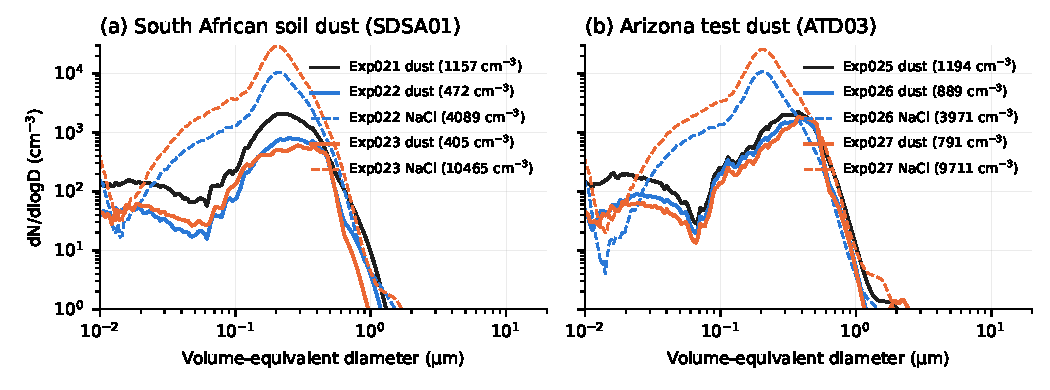
\includegraphics[width=\textwidth]{figs/fig01_aerosol.pdf}
\caption{The mixtures contained less dust than the dust-alone experiments, and the NaCl dominated the number. Initial size distributions of the dust (solid) and NaCl (dashed) components, from KIT's split of the merged SMPS and APS measurements, for (a) SDSA01 and (b) ATD03. Number concentrations in the legend.}
\label{fig:aerosol}
\end{figure}

\begin{figure}[p]
\centering
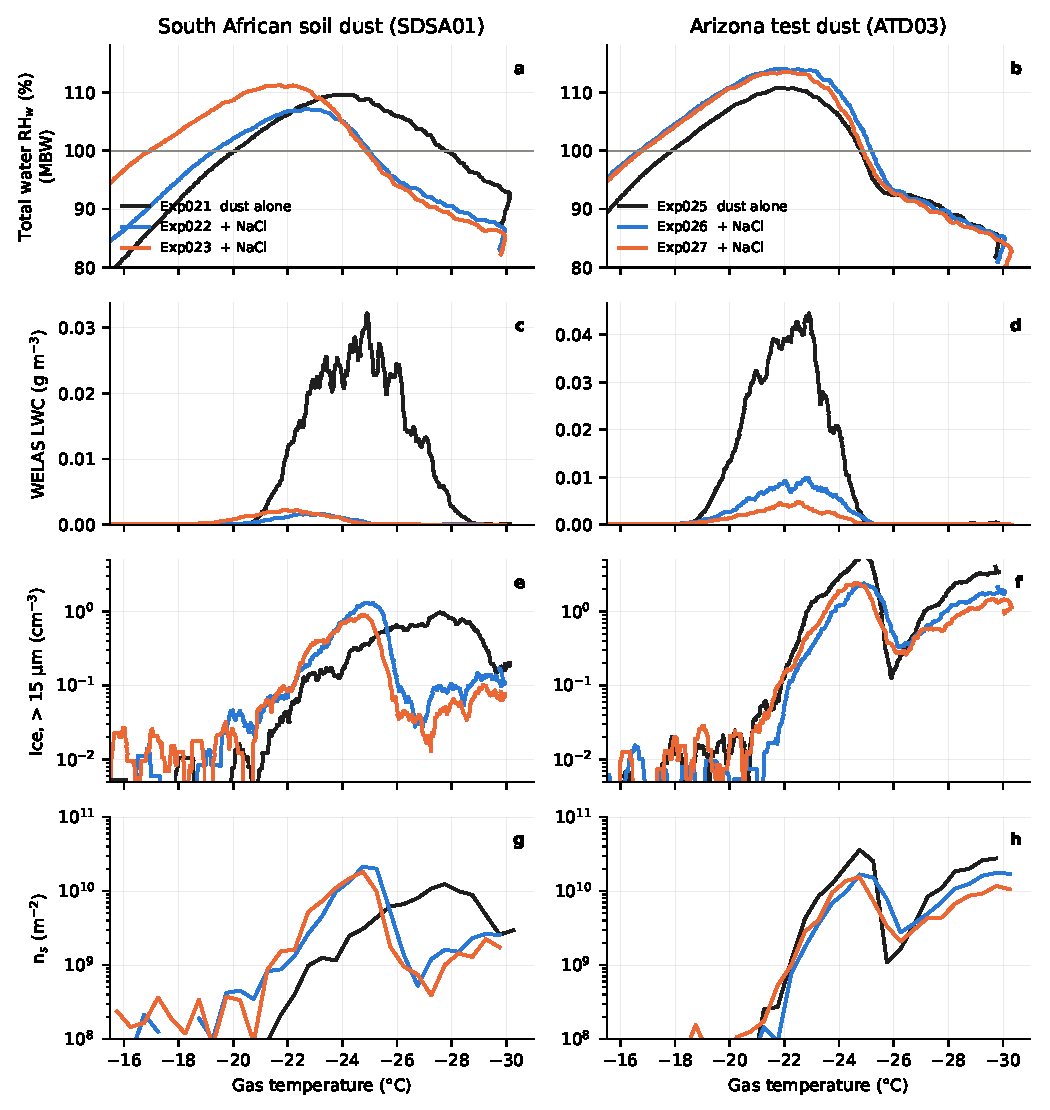
\includegraphics[width=\textwidth]{figs/fig02_observed_overview.pdf}
\caption{With NaCl, WELAS saw little liquid water, but the hygrometer saw the same excess of total water. Observations against gas temperature for (left) SDSA01 and (right) ATD03, alone (black) and mixed with NaCl (blue: about 4000\cmc; orange: about 10\,000\cmc). (a, b) Total water from the MBW hygrometer, as relative humidity over water. (c, d) WELAS liquid water. (e, f) WELAS ice (particles larger than 15\um). (g, h) Ice-nucleation active-site density (Eq.~\ref{eq:ns}), 0.5\,K medians.}
\label{fig:overview}
\end{figure}

\begin{figure}[p]
\centering
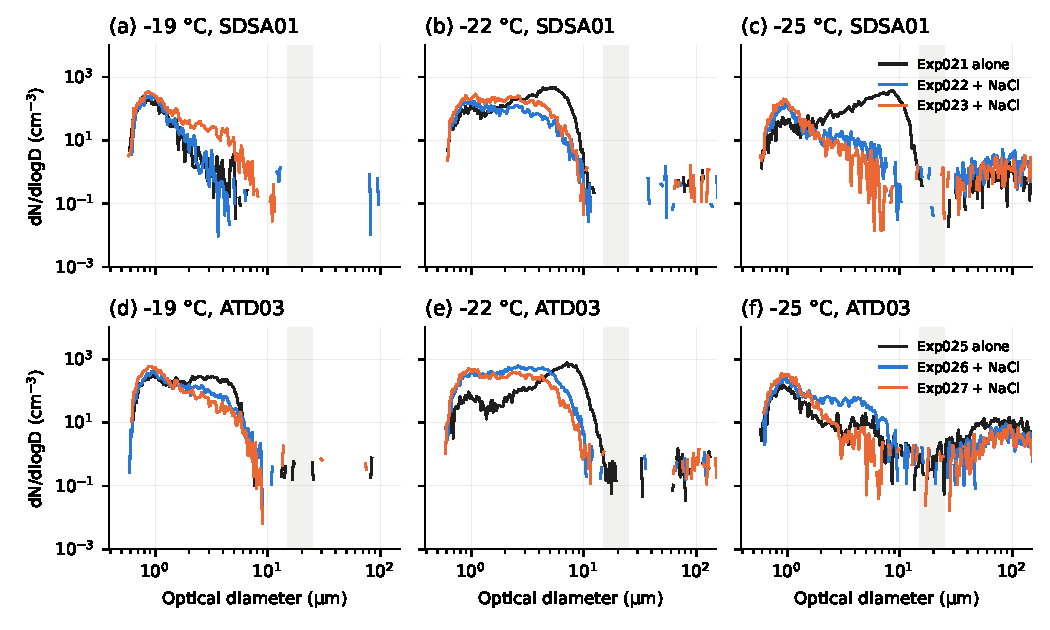
\includegraphics[width=\textwidth]{figs/fig03_welas_spectra.pdf}
\caption{With dust alone a droplet mode formed; with NaCl a broad plateau of 1--7\um\ particles did. WELAS size distributions (30\,s means) as the gas cooled through $-19$, $-22$ and $-25\,^\circ$C, for (a--c) SDSA01 and (d--f) ATD03. Grey band: 15--25\um, between the droplets and the ice.}
\label{fig:spectra}
\end{figure}

\begin{figure}[p]
\centering
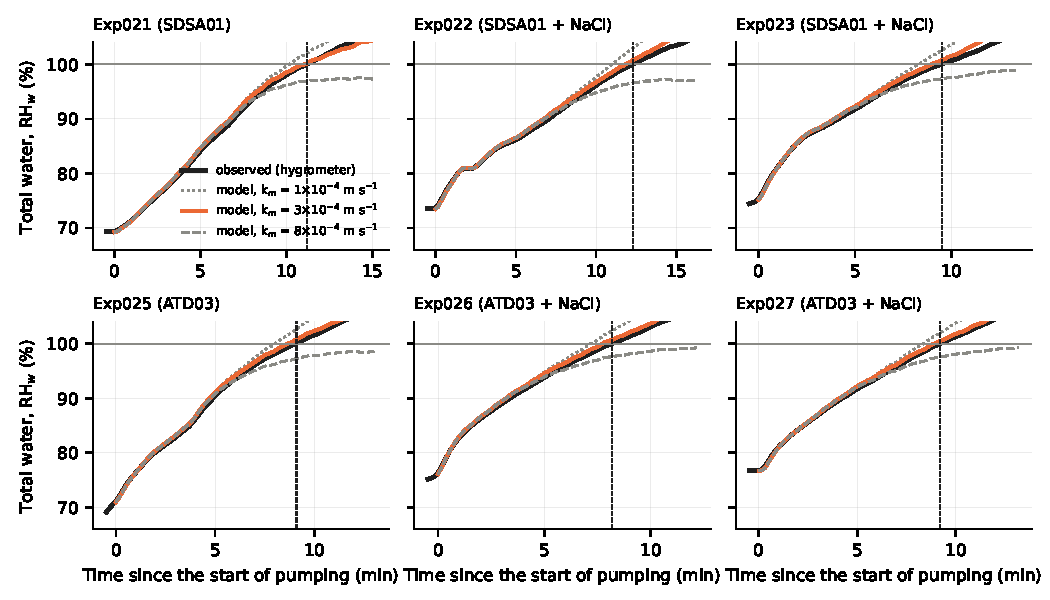
\includegraphics[width=\textwidth]{figs/F04_wall_sink.pdf}
\caption{One rate of water loss to the walls reproduces the total water before the cloud in all six experiments, starting from the measured humidity. Total water as relative humidity over water from the hygrometer (black) and the model with wall transfer velocities $k_\mathrm{m}$ of 1, 3 and $8\times10^{-4}$\,m\,s$^{-1}$ (Eq.~\ref{eq:wallflux}); $3\times10^{-4}$\,m\,s$^{-1}$ is used throughout. Dashed vertical line: $t_\mathrm{sat}$, when the hygrometer reached water saturation.}
\label{fig:wallsink}
\end{figure}

\begin{figure}[p]
\centering
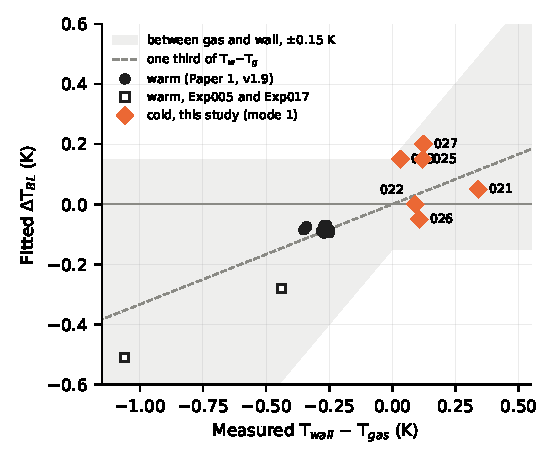
\includegraphics[width=0.55\textwidth]{figs/F05_wall_offsets.pdf}
\caption{The fitted temperature of the wall-conditioned air lies between the gas and the wall temperature in every experiment. Fitted \dTBL\ against the measured wall--gas temperature difference, averaged over the cloud period, for the 14 warm experiments of Paper~1 (circles; open squares: Exp005 without the fan and Exp017 cooled at 4\,K\,min$^{-1}$) and the six cold experiments (diamonds, mode~1). Grey: between the gas and the wall temperature, $\pm0.15$\,K. Dashed: one third of the measured difference. Warm offsets from Paper~1 (v1.9).}
\label{fig:wall}
\end{figure}

\begin{figure}[p]
\centering
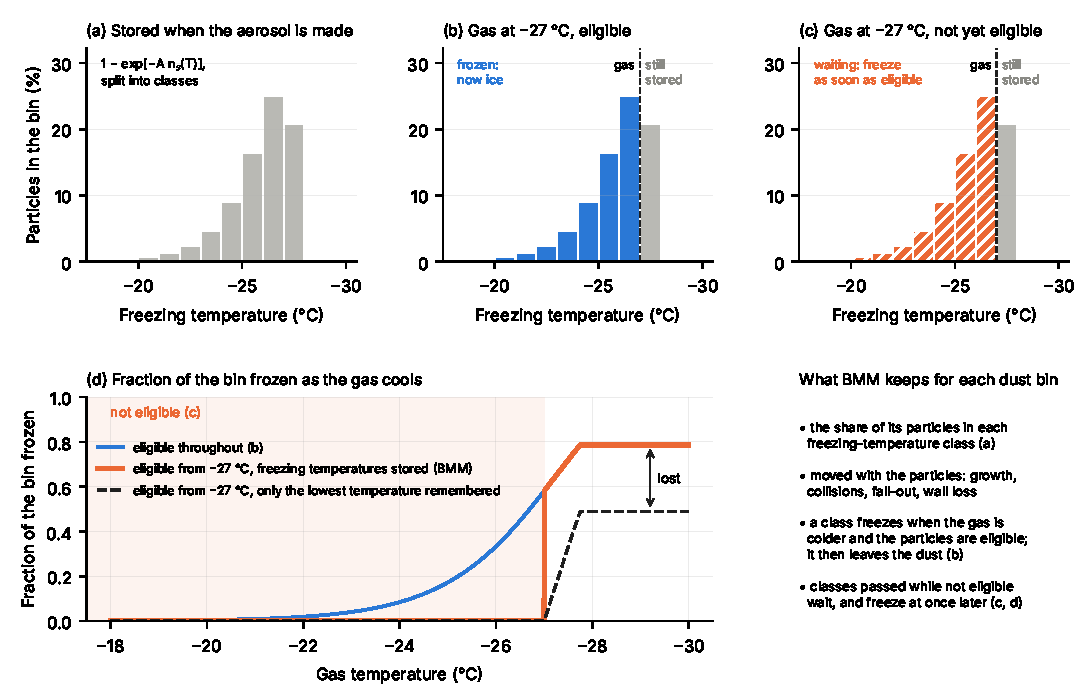
\includegraphics[width=\textwidth]{figs/F06b_ns_scheme.pdf}
\caption{BMM stores the freezing temperatures of the dust in each bin, so that dust cooled past its freezing temperature while it cannot freeze still freezes later. Example: one bin of 2\um\ SDSA01 particles, with \ns\ as used in mode~1; for display the freezing temperatures are grouped into 12 classes of 1\,K (the model uses 100 classes of 0.12\,K). (a) When the aerosol is made, the bin stores the share of its particles in each class, from Eq.~(\ref{eq:inas}); no particle freezes colder than $-27.75\,^\circ$C, where \ns\ is held constant. (b) With the gas at $-27\,^\circ$C and the particles eligible to freeze throughout, every class warmer than the gas has frozen and left the dust (blue). (c) If the particles have not been eligible, the same classes are still stored (hatched); they freeze in the time step in which the particles become eligible. (d) Fraction of the bin frozen as the gas cools: eligible throughout (blue); eligible only from $-27\,^\circ$C with stored freezing temperatures, as in BMM (orange); and eligible only from $-27\,^\circ$C in a scheme that remembers only the lowest temperature reached (dashed), which loses the particles passed while not eligible.}
\label{fig:scheme}
\end{figure}

\begin{figure}[p]
\centering
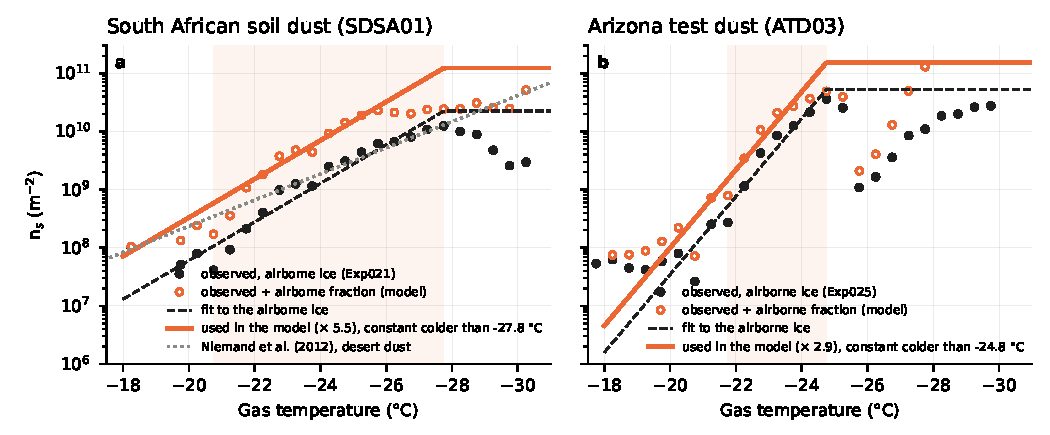
\includegraphics[width=\textwidth]{figs/F06_ns_calibration.pdf}
\caption{The ice-nucleation ability of each dust is taken from its dust-alone experiment and corrected inside the model for crystals that fall out. Observed \ns\ from the airborne ice (black dots, Eq.~\ref{eq:ns}) for (a) Exp021 and (b) Exp025, and the same divided by the airborne fraction of all ice in the calibrated model (open circles). Dashed: fit to the airborne ice over the shaded range. Orange: \ns\ used in the model (mode~1), the fit multiplied by the fall-out factor and held constant colder than the fitted range. Dotted grey: desert-dust fit of \citet{Niemand2012}. Colder than about $-25\,^\circ$C the observed values fall because crystals sediment and, in Exp025, because the liquid has gone.}
\label{fig:ns}
\end{figure}

\begin{figure}[p]
\centering
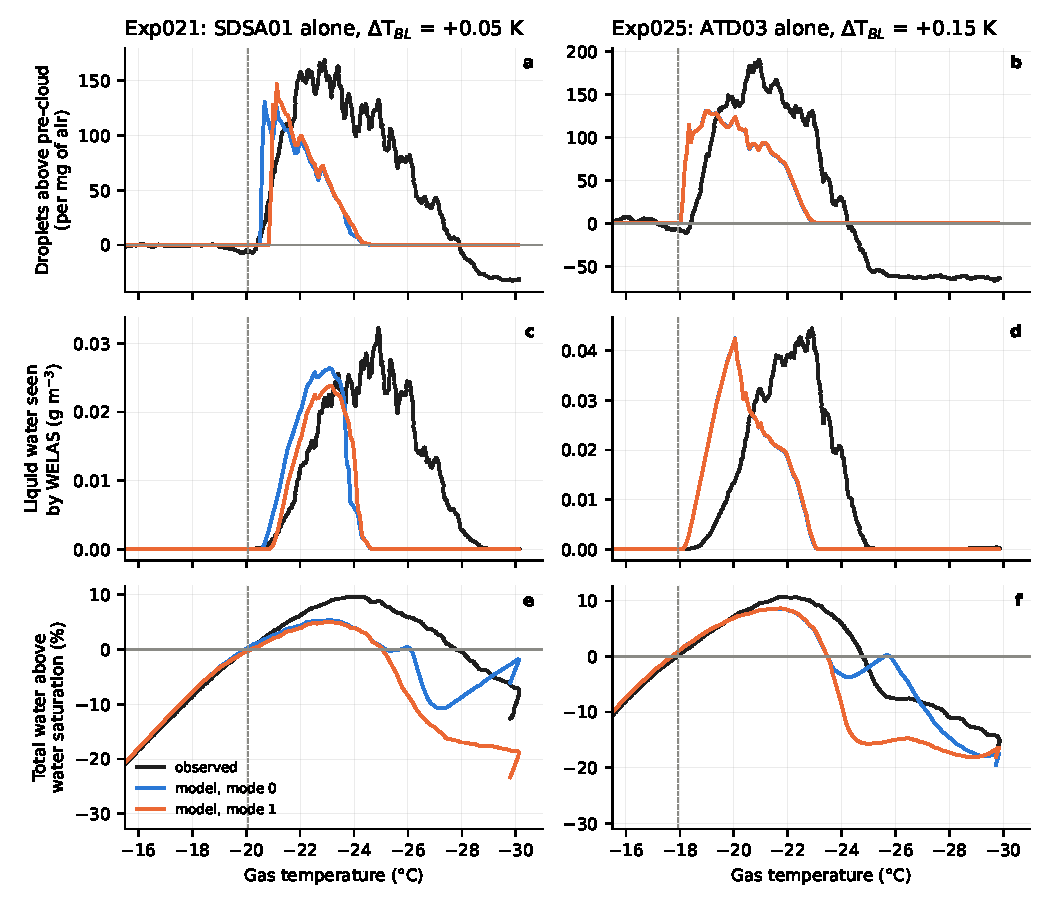
\includegraphics[width=\textwidth]{figs/F07_liquid_dust_alone.pdf}
\caption{The model reproduces the cloud onset, but loses its liquid 1.5--3.5\,K too early, and its total water peaks too low. (a, b) Droplets above the pre-cloud count, per mg of air; (c, d) liquid water; both as WELAS sees them (Eq.~\ref{eq:inlet}). (e, f) Total water above water saturation. Black: observed; blue: model, mode~0; orange: model, mode~1, at the fitted offsets. Dashed vertical line: $t_\mathrm{sat}$.}
\label{fig:liquid}
\end{figure}

\begin{figure}[p]
\centering
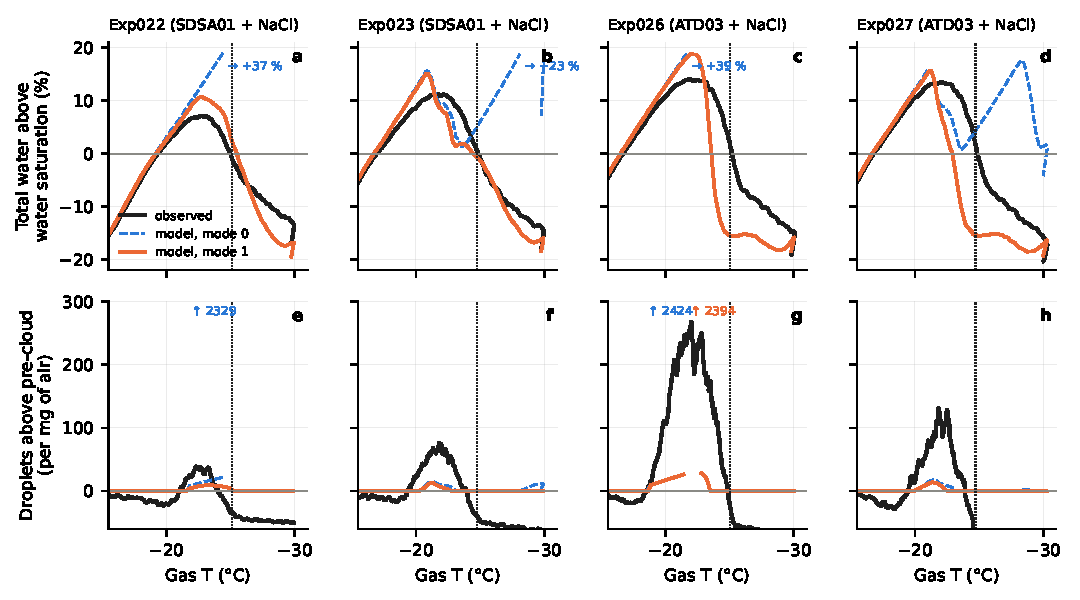
\includegraphics[width=\textwidth]{figs/F08_liquid_mixtures.pdf}
\caption{In the mixtures, only the model in which wetted dust freezes (mode~1) removes the water at glaciation, as observed. (a--d) Total water above water saturation; (e--h) droplets above the pre-cloud count visible to WELAS, per mg of air. Black: observed; dashed blue: model, mode~0; orange: model, mode~1; each mode at its own fitted offset. Model values beyond the axes are given as numbers. Dotted vertical line: observed end of the liquid phase.}
\label{fig:liquidmix}
\end{figure}

\begin{figure}[p]
\centering
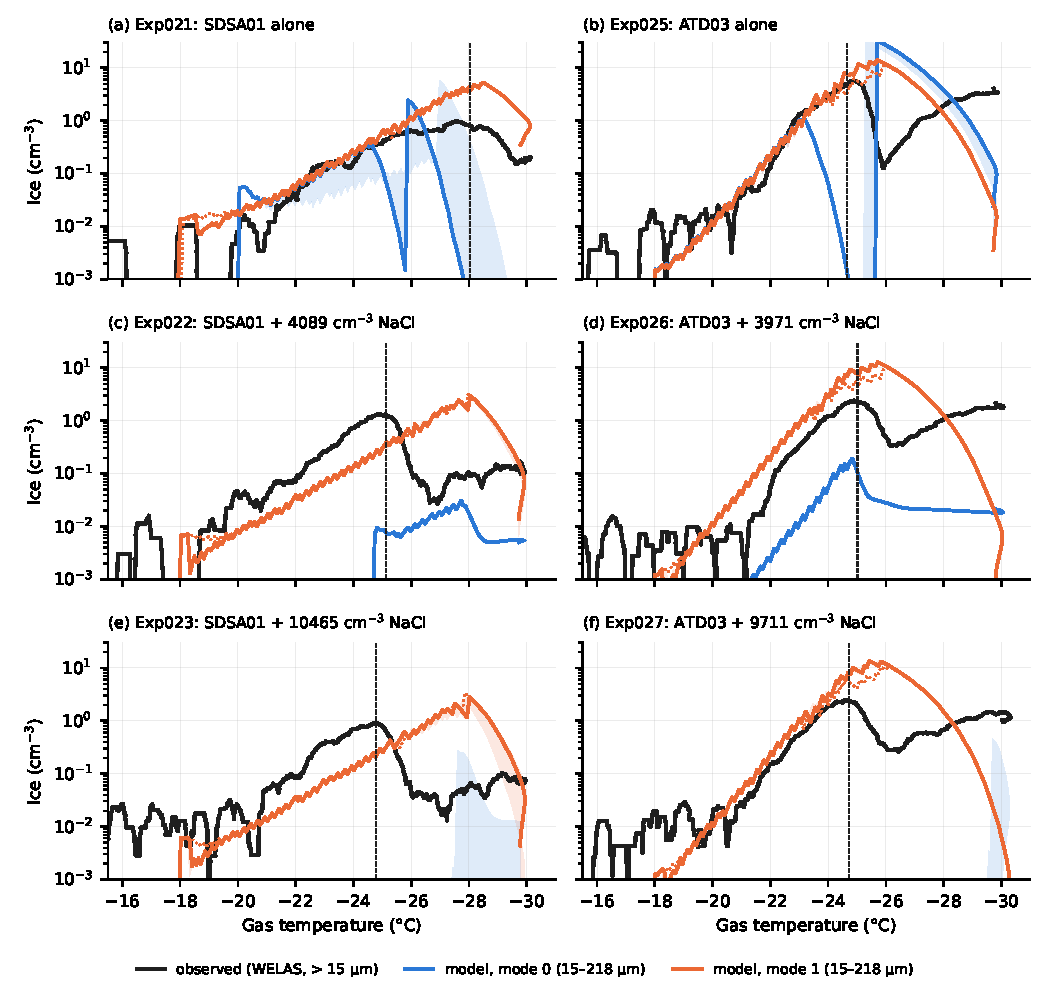
\includegraphics[width=\textwidth]{figs/F09_ice.pdf}
\caption{If dust must activate to freeze (mode~0, blue), NaCl almost stops ice formation in the model; if wetted dust can freeze (mode~1, orange), it does not. Ice against gas temperature from WELAS (black; particles larger than 15\um, 61\,s means) and the model (crystals of 15--218\um\ by projected-area-equivalent diameter; dotted: volume-equivalent diameter, mode~1) at the fitted offsets; shading: all acceptable fits. Dashed vertical line: observed end of the liquid phase; after it the observed ice falls and the model's does not. Rows: dust alone, with about 4000\cmc\ NaCl, with about 10\,000\cmc\ NaCl. Columns: SDSA01, ATD03.}
\label{fig:ice}
\end{figure}

\begin{figure}[p]
\centering
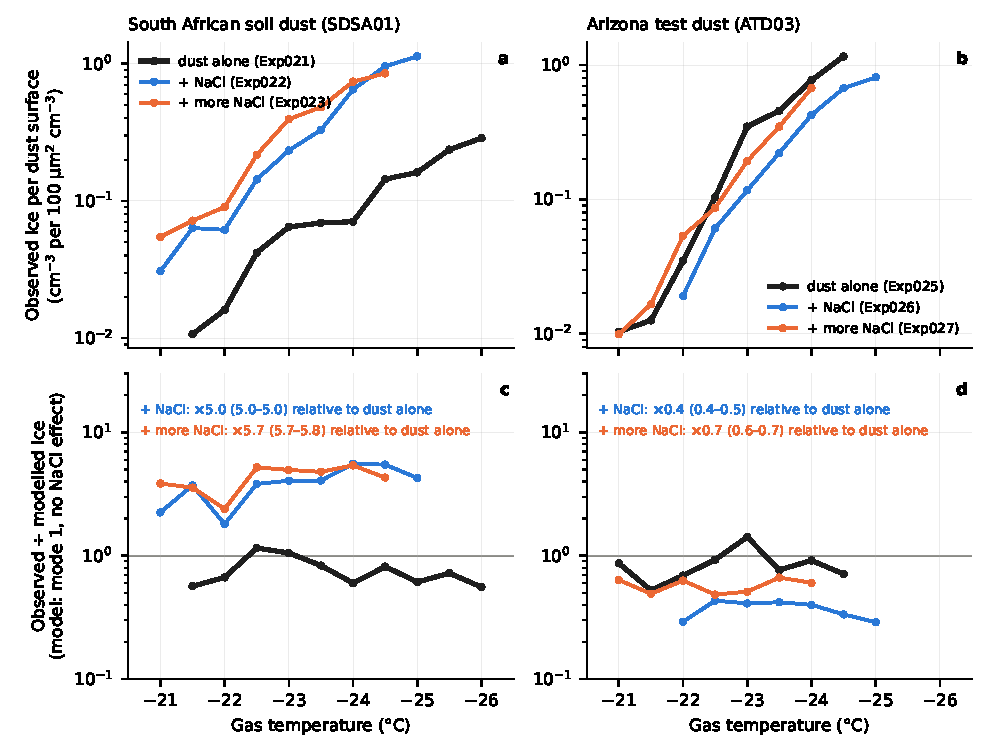
\includegraphics[width=\textwidth]{figs/F10_matched_T.pdf}
\caption{At the same temperature, the SDSA01 mixtures formed five to six times more ice per unit dust surface than the dust alone, and the ATD03 mixtures about half as much. (a, b) Observed ice per unit initial dust surface against gas temperature, before glaciation. (c, d) Observed over modelled ice, with the model in mode~1, which contains no effect of the NaCl on freezing; the residual effect $E$ (Eq.~\ref{eq:E}) is given with its range over all acceptable fits.}
\label{fig:matched}
\end{figure}

\begin{figure}[p]
\centering
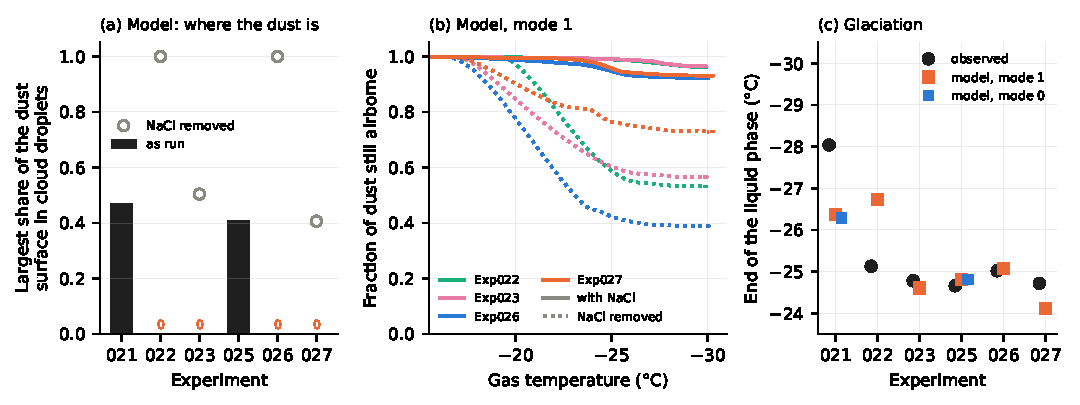
\includegraphics[width=\textwidth]{figs/F11_mechanisms.pdf}
\caption{With NaCl none of the dust activates in the model, and the dust stays airborne. (a) Largest share of the airborne, unfrozen dust surface in cloud droplets (wet diameter above 2\um) between $t_\mathrm{sat}$ and the end of the liquid phase, mode~1, as run (bars) and with the NaCl removed (open circles). (b) Fraction of the dust still airborne (in haze, droplets or ice) in mode~1, with NaCl (solid) and with the NaCl removed (dotted). (c) Gas temperature at which the liquid water fell below 10\,\% of its peak: observed (black), mode~1 (orange) and mode~0 (blue; the mixtures do not glaciate in mode~0).}
\label{fig:mechanisms}
\end{figure}

\begin{figure}[p]
\centering
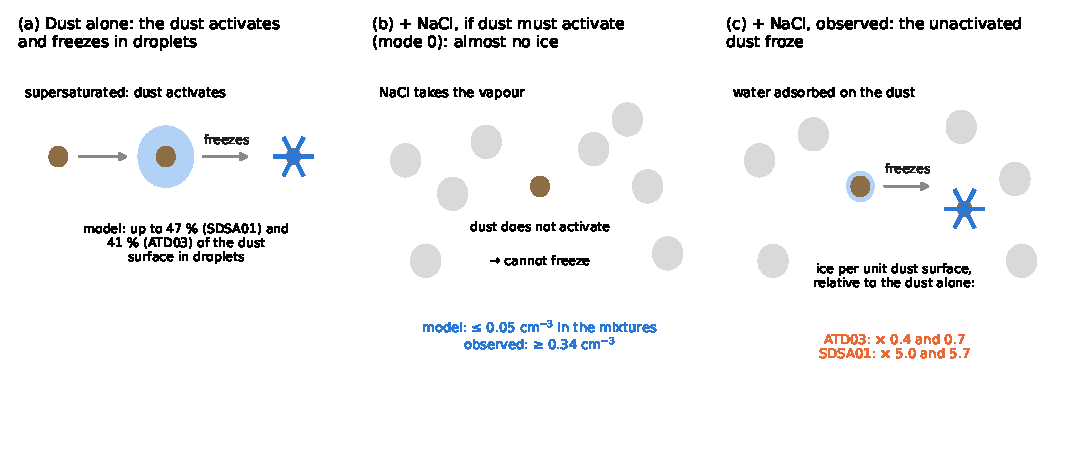
\includegraphics[width=\textwidth]{figs/F12_schematic.pdf}
\caption{How NaCl changes ice formation on dust. (a) Dust alone: the dust activates, and the droplets freeze. (b) With NaCl, the NaCl takes the vapour and the dust stays unactivated; if dust must activate to freeze (mode~0), almost no ice forms. (c) Observed: the unactivated dust froze, at about half the rate of the dust alone for ATD03 and five to six times the rate for SDSA01, per unit dust surface at the same temperature.}
\label{fig:schematic}
\end{figure}
